\section{Синтез регулятора с заданной степенью устойчивости}

\subsection{Анализ системы} \label{sec:anal1}

Рассмотрим систему
\begin{equation}
    \dot x=Ax+Bu,\quad A=\begin{bmatrix}
        3&5&4\\
        -2&-4&-5\\
        2&2&3
    \end{bmatrix},\quad B=\begin{bmatrix}
        2\\-1\\1
    \end{bmatrix}.
    \label{eq:sys1}
\end{equation}
Cобственные числа матрицы $A$
\begin{equation*}
    \sigma(A)=\{\ 2\pm i,\ -2\ \}.
\end{equation*}
Рассмотрим матрицы Хаутуса и их ранги
\begin{equation*}
    H_1 = \begin{bmatrix}
        (2+ i) I - A & B
    \end{bmatrix} =
    \begin{bmatrix}
        -1 + i & -5 & -4 & 2 \\ 
         2 &  6 + i &  5 & -1 \\ 
        -2 & -2 & -1 + i &  1
    \end{bmatrix},
    \quad\text{rank}(H_1) = 3,
\end{equation*}
\begin{equation*}
    H_2 = \begin{bmatrix}
        (2- i) I - A & B
    \end{bmatrix} =
    \begin{bmatrix}
        -1 - i & -5 & -4 & 2 \\ 
         2 &  6 - i &  5 & -1 \\ 
        -2 & -2 & -1 - i &  1
    \end{bmatrix},
    \quad\text{rank}(H_2) = 3,
\end{equation*}
\begin{equation*}
    H_3 = \begin{bmatrix}
        -2 I - A & B
    \end{bmatrix} =
    \begin{bmatrix}
        -5 & -5 & -4 &  2 \\ 
         2 &  2 &  5 & -1 \\ 
        -2 & -2 & -5 &  1
    \end{bmatrix},
    \quad\text{rank}(H_3) = 2.
\end{equation*}
Как видно, система не полностью управляема, но стабилизируема, так как единственное
неуправляемое собственное число $-2$ отрицательно.

Если мы будем использовать регулятор вида $u=Kx$, то не получится получить
любую степень устойчивости, так как система не полностью управляема, и
более $-2$ степени устойчивости не получится, она максимальна, снизу число ограничено 
только определением, а именно нулем.

Построим схему моделирования (см. \autoref{fig:sys1}) системы \eqref{eq:sys1} с регулятором $u=Kx$.
\begin{figure}[H]
    \centering
    \caption{Схема моделирования системы \eqref{eq:sys1} с регулятором $u=Kx$}
    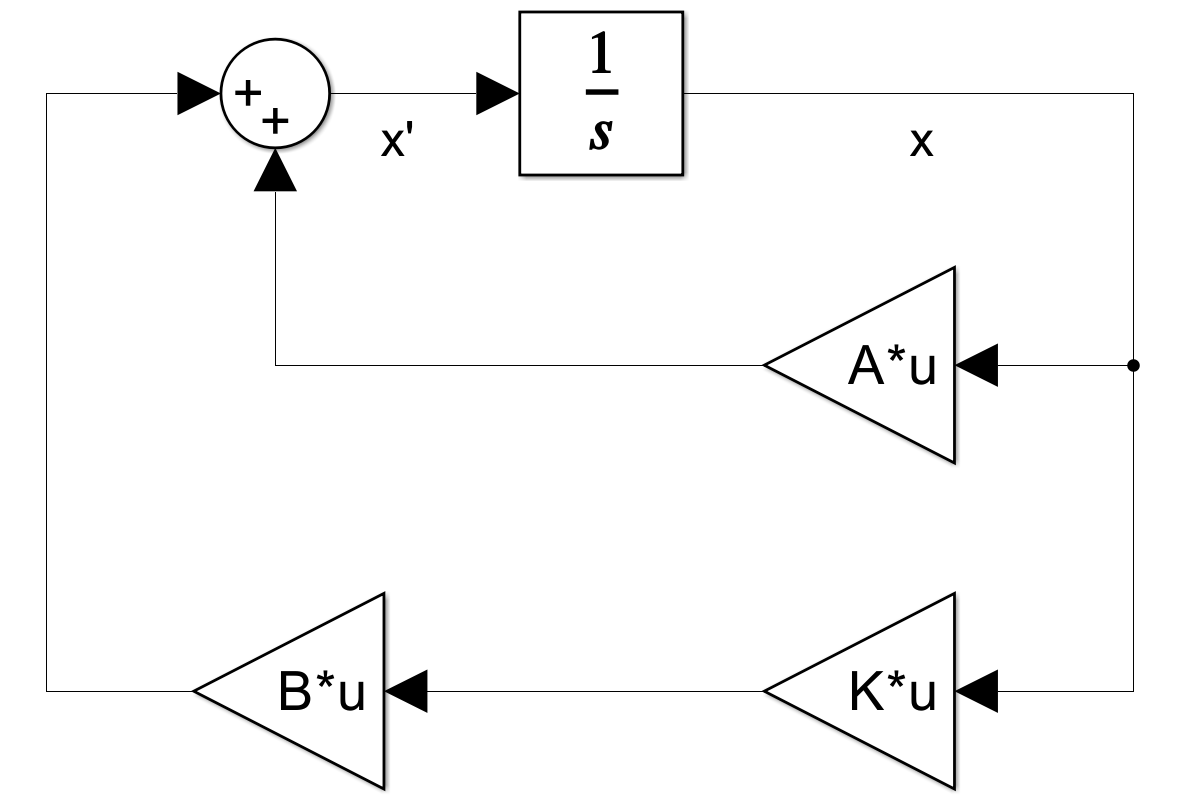
\includegraphics[width=0.8\textwidth]{figs/task1_slx.png}
    \label{fig:sys1}
\end{figure}

Зададимся парой значений степени устойчивости $\alpha_1=2$ и $\alpha_2=0.2$
для дальнейшего их исследования.



\subsection{Степень устойчивости 1}

\subsubsection{Синтез регулятора при помощи матричного неравенства
типа Ляпунова} \label{sec:lyapexp}

Синтезируем регулятор со степенью устойчивости $\alpha_1=2$ при помощи
матричного неравенства типа Ляпунова
\begin{equation}
    PA^T+AP+2\alpha P+Y^TB^T+BY\preccurlyeq0,\quad P\succ0,\quad K=YP^{-1}.
    \label{eq:lyap}
\end{equation}
Найдем матрицу регулятора $K_1$, обеспечивающую желаемую степень 
устойчивости без ограничений на управление, для этого воспользуемся CVX, 
используя неравенства \eqref{eq:lyap}. Получаем
\begin{equation*}
    K_1=\begin{bmatrix}
        3.3536&	2.1216&	-17.9071
    \end{bmatrix}.
\end{equation*}
Найдем матрицу регулятора $K_2$, обеспечивающую желаемую степень 
устойчивости совместно с решением задачи минимизации управления,
для этого понадобятся еще пара неравенств:
\begin{equation}
    \begin{bmatrix}
        P&x_0\\
        x_0^T&1
    \end{bmatrix}\succ0,\quad
    \begin{bmatrix}
        P&Y^T\\
        Y&\gamma I
    \end{bmatrix}\succ0,
\end{equation}
минимизировать нужно $\gamma$, начальное состояние возьмем 
нулевым (оно большой роли не играет, насколько я понимаю), и, используя CVX, получим
\begin{equation*}
    K_2=\begin{bmatrix}
        -1.0712&	-1.0712&	-3.3288
    \end{bmatrix}.
\end{equation*}


\subsubsection{Синтез регулятора при помощи матричного
уравнения типа Риккати}

Уравнение Риккати выглядит следующим образом
\begin{equation}
    A^TP+PA+Q-vPBR^{-1}B^TP+2\alpha P=0,\quad K=-R^{-1}B^TP
\end{equation}
при этом для работы регулятора необходимо $P\succ0$. Нас интересует его форма когда
$v=2$ и $R=1,$ тогда уравнение выглядит следующим образом
\begin{equation}
    A^TP+PA+Q-2PBB^TP+2\alpha P=0,\quad K=-B^TP.
    \label{eq:ric}
\end{equation}
Находить решение будем через vpasolve, а для этого нужно ``урезать'' систему,
чтобы она стала полностью управляемой. Жорданова форма систему выглядит
следующим образом
\begin{equation}
    A_J=\begin{bmatrix}
        -2&0&0\\
        0&2&-1\\
        0&1&2
    \end{bmatrix},\quad
    B_J=\begin{bmatrix}
        0\\0.7071\\-2.1213
    \end{bmatrix},\quad
    P=\begin{bmatrix}
        -1&	0.7071&	-0.7071\\
        1&	-1.4142&	0\\
        0&	1.4142&	0
    \end{bmatrix}.
    \label{eq:sys1jourdan}
\end{equation}
``Урезанная'' версия:
\begin{equation}
    A_j=\begin{bmatrix}
        2&-1\\
        1&2
    \end{bmatrix},\quad
    B_j=\begin{bmatrix}
        0.7071\\-2.1213
    \end{bmatrix}
    \label{eq:sys1j}
\end{equation}
Теперь с помощью vpasolve найдем матрицу регулятора, решив уравнение \ref{eq:ric}
и взяв за $Q$ единичную матрицу,
\begin{equation*}
    K_{3_j}=\begin{bmatrix}
        16.6595& -1.5221
    \end{bmatrix},
\end{equation*}
дополним ее
\begin{equation*}
    K_{3_J}=\begin{bmatrix}
        0&16.6595& -1.5221
    \end{bmatrix},
\end{equation*}
и найдем ее в исходном базисе
\begin{equation*}
    K_3=K_{3_J}P^{-1}=\begin{bmatrix}
        2.1526&2.1526& -10.7037
    \end{bmatrix}.
\end{equation*}
Теперь возьмем за $Q$ нулевую матрицу, было найдено решение
\begin{equation*}
    K_{4_j}=\begin{bmatrix}
        -14.7078& -1.1314
    \end{bmatrix},
\end{equation*}
найдем матрицу в исходном базисе
\begin{equation*}
    K_4=K_{4_J}P^{-1}=\begin{bmatrix}
        1.6&1.6& -9.6
    \end{bmatrix}.
\end{equation*}



\subsubsection{Проверка регуляторов}

Найдем собственные числа матриц замкнутых систем
\begin{equation*}
    \sigma(A+BK_1)=\{\ -4.6608 \pm 3.6560i,\ -2\ \},\quad
    \sigma(A+BK_2)=\{\ -2 \pm 2.8798i,\ -2\ \},
\end{equation*}
\begin{equation*}
    \sigma(A+BK_3)=\{\ -2.2755 \pm 4.3745i,\ -2\ \},\quad
    \sigma(A+BK_4)=\{\ -2 \pm 4.1231i,\ -2\ \}.
\end{equation*}
Как видно, система стала устойчивой с желаемой степенью в каждом случае. При нахождении 
регулятора при помощи матричного неравенства типа Ляпунова без ограничения управления 
($K_1$) собственные числа получились какие-то ``случайные''
и даже более ``устойчивые'' чем требуется; при минимизации управления ($K_2$), собственные
числа подобрались минимально возможные для удовлетворения желаемой степени устойчивости.
Если посмотреть на регуляторы, получившиеся из решения уравнения Риккати, заметим, что
оба спектра при $K_3$ и $K_4$ очень похожи, и далее на графиках будет видно, что система с данными
регуляторами ведет себя одинакого, но в тоже время заметим, что при $Q=0$ управление
потребуется меньше, чем при $Q=I$.




\subsubsection{Моделирование}

Для четырех замкнутых систем выполним компьютерное моделирование,
построим графики формируемых регуляторами управлений $u(t)$ и векторов
состояния замкнутых систем $x(t)$ при начальных условиях $x(0) =\begin{bmatrix}
    1&1&1
\end{bmatrix}^T$ (см \autoref{fig:1k1}). Как видно по графикам, управление
при регуляторе $K_2$, который синтезировался с ограничением управления, менее
``сильное'' в сравнении с регулятором $K_1$, что заметно отражается на 
скорости сходимости состояния к точке равновесия. Сравнивая же эти регуляторы,
найденные из матричного неравенства типа Ляпунова, с регуляторами, найденными
из решения уравнения типа Риккати, замечу, что по ``силе'' управления, времени
сходимости и перерегулировании они получились средние, то есть 
$K_1$ и $K_2$ - крайности, а $K_3$ и $K_4$ ``сидят'' где-то между ними,
никак не выделяясь. Сравнивать их между собой смысла не вижу, так как и по 
графикам управления, и по графикам состояний они крайне похожи.

\begin{figure}[H]
    \centering
    \caption{Моделирование системы \eqref{eq:sys1} с регулятором вида $u=Kx$
    со степенью устойчивости $\alpha=2$}
    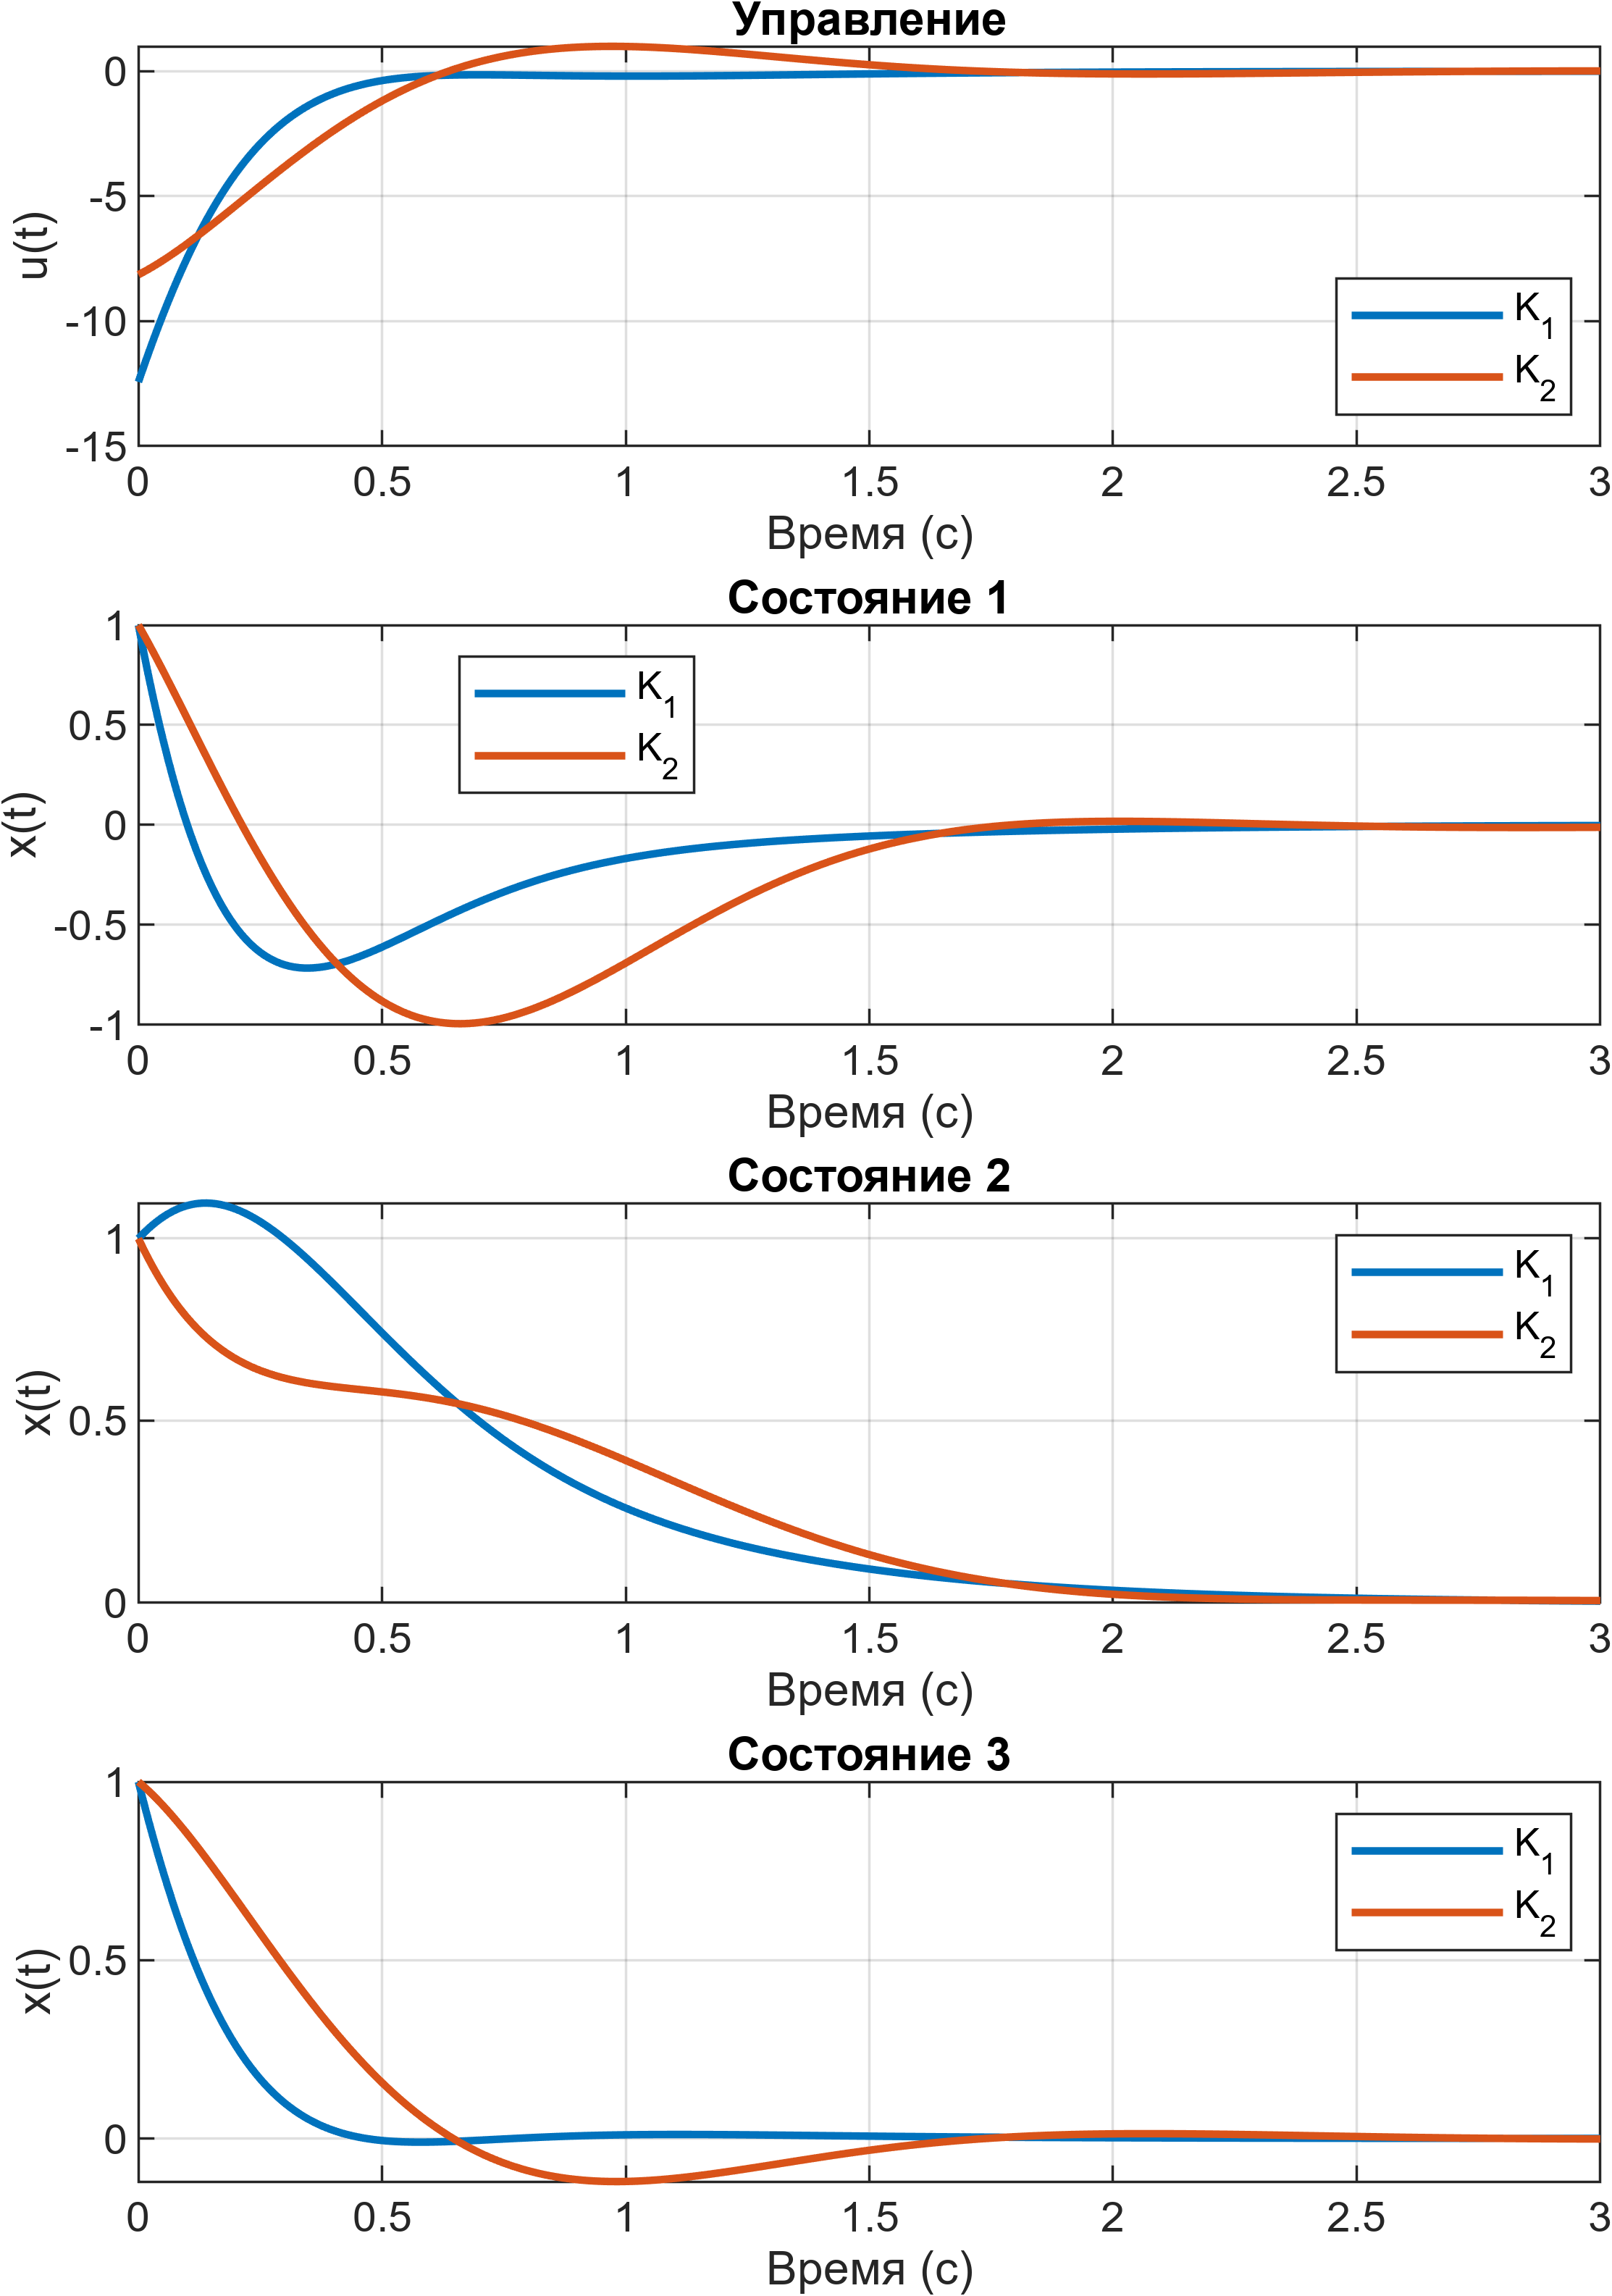
\includegraphics[width=\linewidth]{figs/task10.png}
    \label{fig:1k1}
\end{figure}




\subsection{Степень устойчивости 2}

\subsubsection{Синтез регулятора при помощи матричного неравенства
типа Ляпунова}

Аналогично синтезируем регулятор со степенью устойчивости $\alpha_1=0.2$.
Найдем матрицу регулятора $K_1$, обеспечивающую желаемую степень 
устойчивости без ограничений на управление, для этого воспользуемся CVX и получим
\begin{equation*}
    K_1=\begin{bmatrix}
        -1.6329&	-2.3204&	-9.5054
    \end{bmatrix}.
\end{equation*}
Найдем матрицу регулятора $K_2$, обеспечивающую желаемую степень 
устойчивости совместно с решением задачи минимизации управления,
начальное состояние так же возьмем нулевым, и, используя CVX, получим
\begin{equation*}
    K_2=\begin{bmatrix}
        -1.0712&	-1.0712&	-3.3288
    \end{bmatrix}.
\end{equation*}


\subsubsection{Синтез регулятора при помощи матричного
уравнения типа Риккати}

Аналогично находим решение через vpasolve, решив уравнение \ref{eq:ric}
и взяв за $Q$ единичную матрицу, получим
\begin{equation*}
    K_{3_j}=\begin{bmatrix}
        -6.4311& 0.3254
    \end{bmatrix},
\end{equation*}
дополним ее
\begin{equation*}
    K_{3_J}=\begin{bmatrix}
        0&-6.4311& 0.3254
    \end{bmatrix},
\end{equation*}
и найдем в исходном базисе
\begin{equation*}
    K_3=K_{3_J}P^{-1}=\begin{bmatrix}
        -0.4603& -0.4603& -4.7777
    \end{bmatrix}.
\end{equation*}
Теперь возьмем за $Q$ нулевую матрицу, было найдено решение
\begin{equation*}
    K_{4_j}=\begin{bmatrix}
        -4.7291& 0.4978
    \end{bmatrix},
\end{equation*}
найдем матрицу в исходном базисе
\begin{equation*}
    K_4=K_{4_J}P^{-1}=\begin{bmatrix}
        -0.704& -0.704& -3.696
    \end{bmatrix}.
\end{equation*}


\subsubsection{Проверка регуляторов}

Найдем собственные числа матриц замкнутых систем
\begin{equation*}
    \sigma(A+BK_1)=\{\ -1.4599,\    -4.9909,\    -2\ \},\quad
    \sigma(A+BK_2)=\{\ -0.2 \pm 2.0010i,\ -2\ \}.
\end{equation*}
\begin{equation*}
    \sigma(A+BK_3)=\{\ -0.6190 \pm 2.7484i\  -2\ \},\quad
    \sigma(A+BK_4)=\{\ -0.2 \pm 2.4166i,\ -2\ \}.
\end{equation*}
Как видно, система стала устойчивой с желаемой степенью. Результат
абсолютно аналогичен, когда за желаемую степень устойчивости принималось число 2.
Все также при занулении $Q$ нашлось решение, которое имеет вещественные
части у спектра замкнутой системы равным минимально возможным, чтобы
удовлетворялась желаемая степень устойчивости.


\subsubsection{Моделирование}

Для четырех замкнутых систем выполним компьютерное моделирование,
построим графики формируемых регуляторами управлений $u(t)$ и векторов
состояния замкнутых систем $x(t)$ при начальных условиях $x(0) =\begin{bmatrix}
    1&1&1
\end{bmatrix}^T$ (см \autoref{fig:2k1}). Выводы аналогичны таковым при степени
устойчивости 2, разве что самое плохое перерегулирование теперь имеет система при
$K_4$, и в этот раз системы с регуляторами $K_3$ И $K_4$
не очень похожи и имеют различающиеся графики управления и состояния. Это 
связано с тем что в этот раз спектры соответствующих замкнуных систем отличаются
гораздо сильнее.


\subsection{Выводы}

Были синтезированы регуляторы с заданными степенями устойчивости. 
Использовались два подхода: матричное неравенства типа Ляпунова и 
матричное уравнение Риккати. Оба метода показали свою эффективность, обеспечив желаемую 
степень устойчивости. Однако, регуляторы, найденные через Ляпунова, продемонстрировали 
крайние значения управления, в то время как регуляторы из Риккати оказались более 
средними. Моделирование подтвердило корректность синтеза.


\begin{figure}[H]
    \centering
    \caption{Моделирование системы \eqref{eq:sys1} с регулятором вида $u=Kx$
    со степенью устойчивости $\alpha=0.2$}
    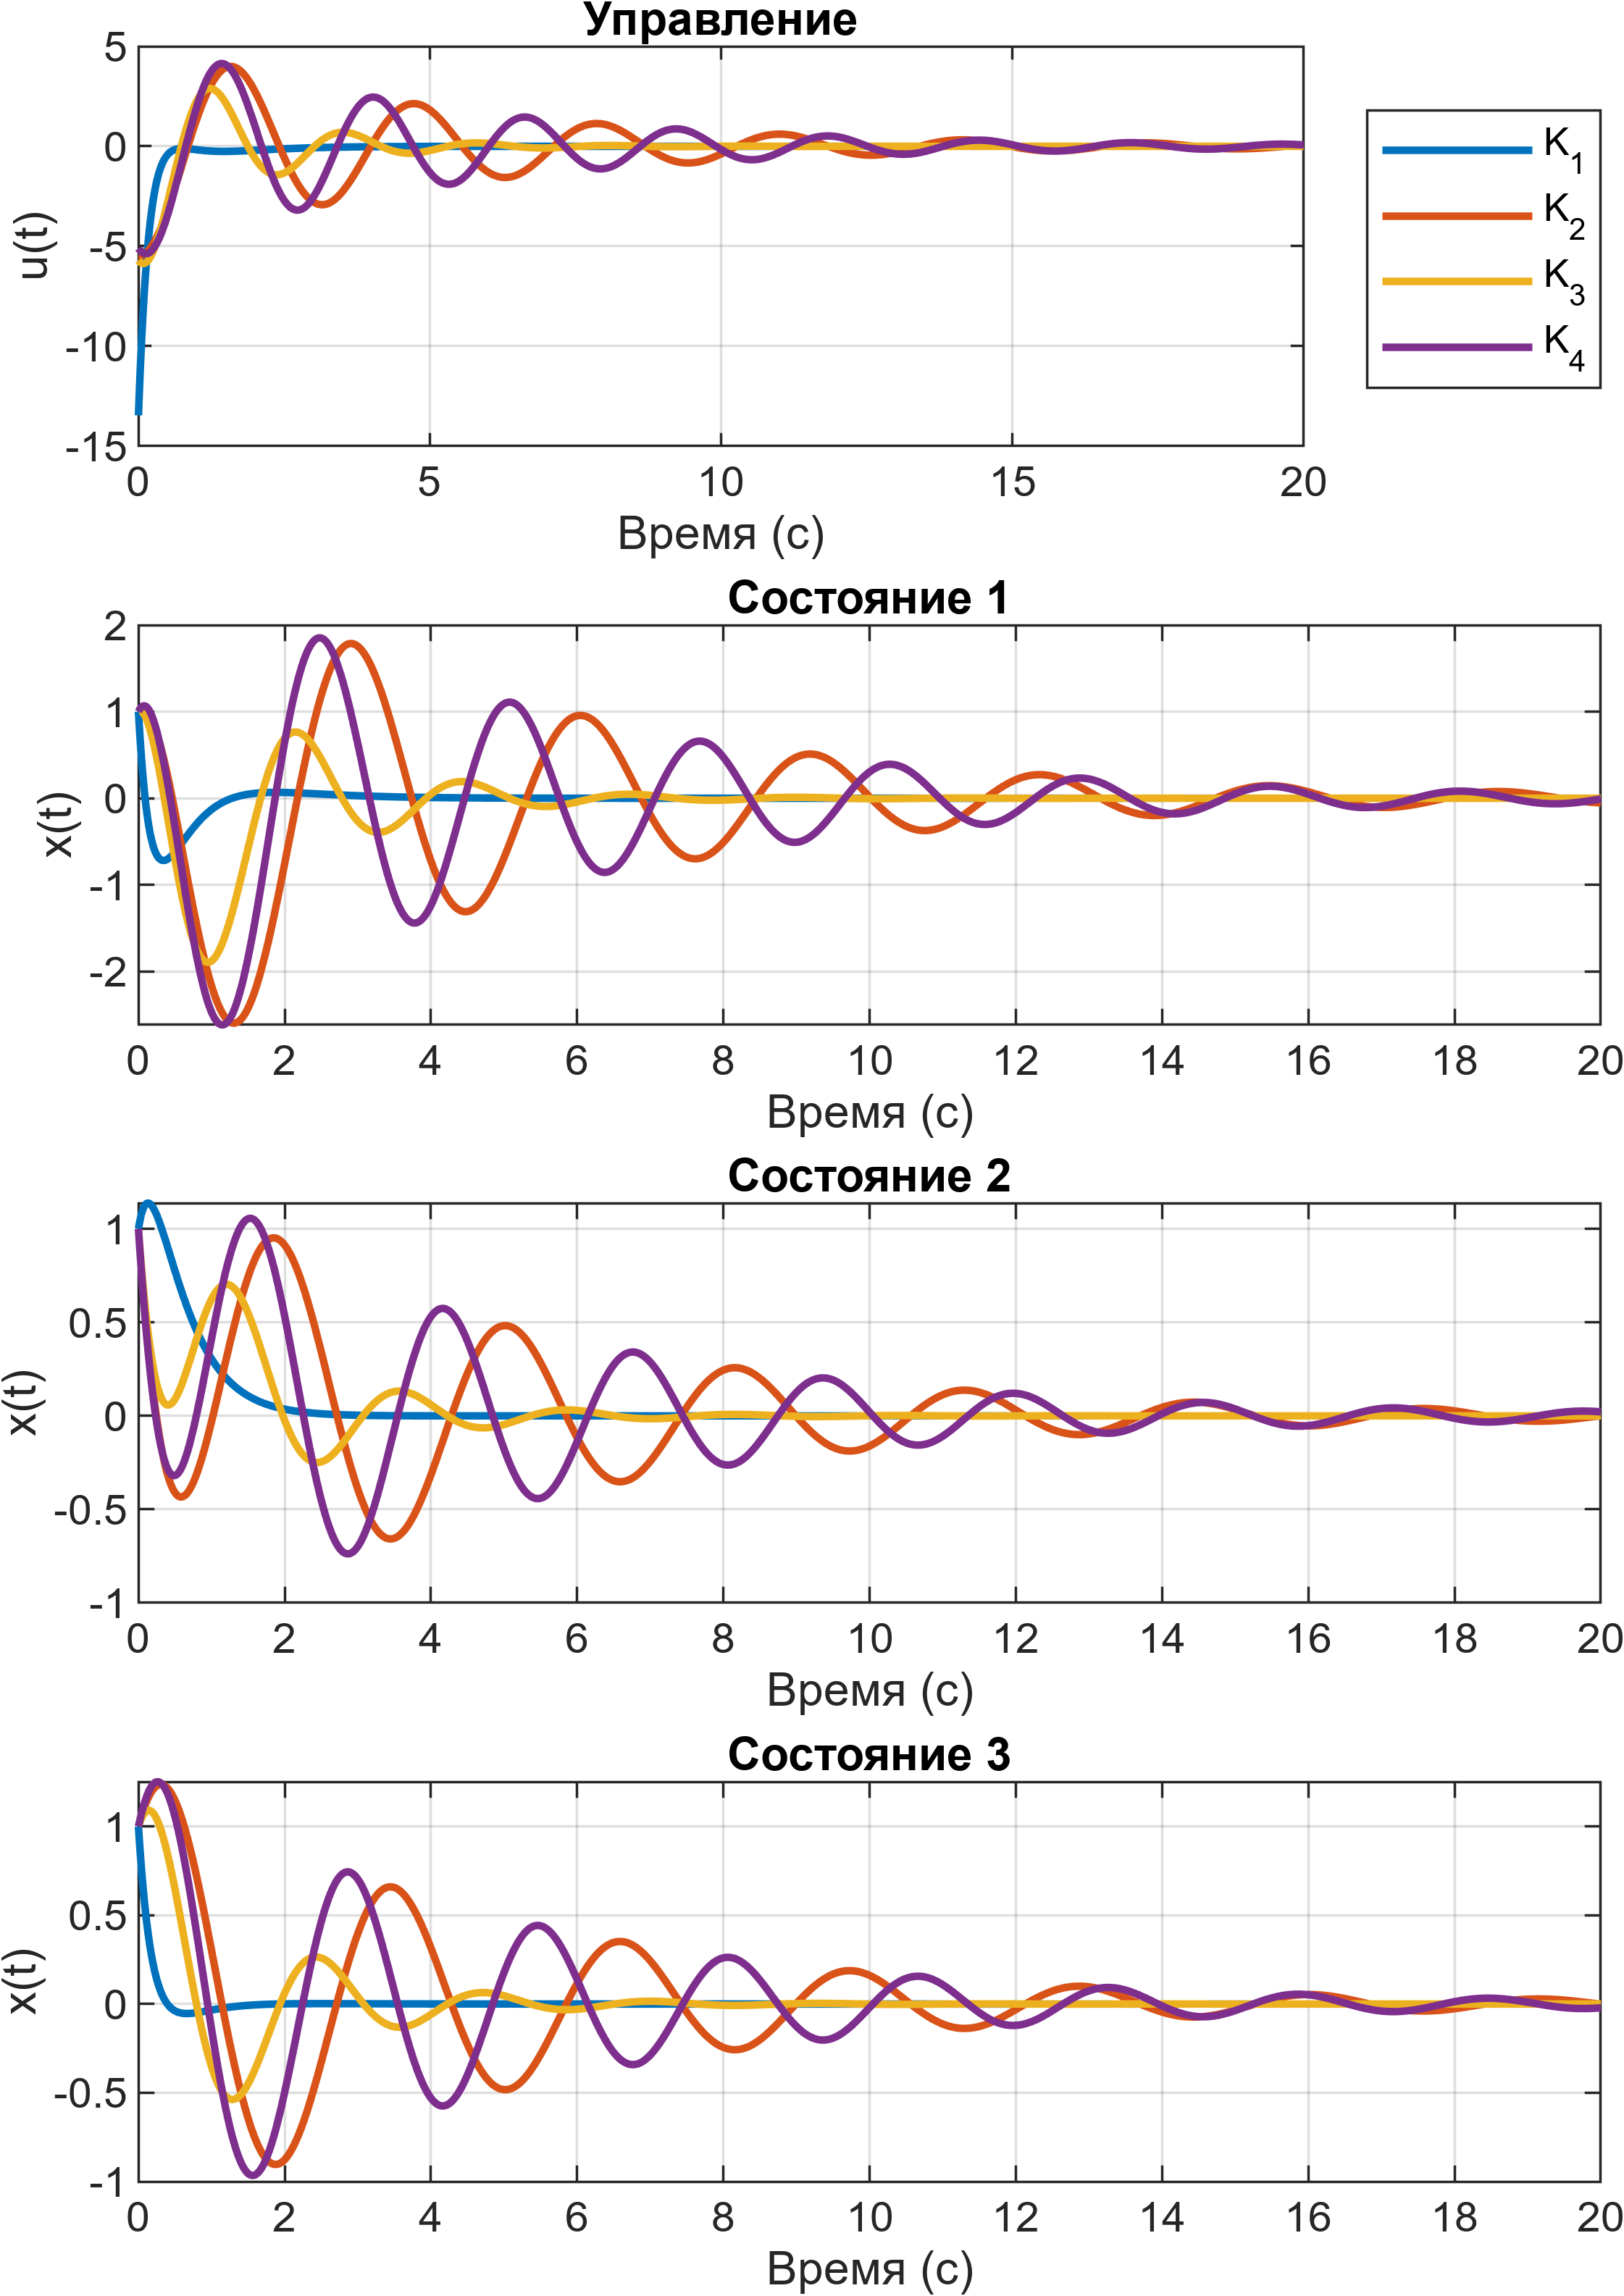
\includegraphics[width=\linewidth]{figs/task11.png}
    \label{fig:2k1}
\end{figure}





\section{Управление по выходу с заданной степенью устойчивости}

\subsection{Анализ системы}

Рассмотрим систему
\begin{equation}
    \begin{cases}
        \dot x=Ax+Bu,\\
        y=Cx,
    \end{cases}\quad
    A=\begin{bmatrix}
        5&-5&-9&3\\
        -5&5&-3&9\\
        -9&-3&5&5\\
        3&9&5&5
    \end{bmatrix},\quad 
    B=\begin{bmatrix}
        2\\6\\6\\2
    \end{bmatrix},\quad
    C=\begin{bmatrix}
        1&-1&1&1\\
        1&3&-1&3
    \end{bmatrix}.
    \label{eq:sys2}
\end{equation}
Спектр матрицы $A$
\begin{equation*}
    \sigma(A)=\{ -12,\ 4,\ 12,\ 16 \}.
\end{equation*}
Составим матрицы Хаутуса
\begin{equation*}
    H_1 = \begin{bmatrix}
        -12 I - A & B
    \end{bmatrix} =
    \begin{bmatrix}
        -17 & 5  & 9  & -3 & 2  \\
         5  & -17 & 3  & -9 & 6  \\
         9  & 3  & -17 & -5 & 6  \\
        -3  & -9 & -5  & -17 & 2
    \end{bmatrix},
    \quad\text{rank}(H_1) = 4,
\end{equation*}
\begin{equation*}
    H_2 = \begin{bmatrix}
        4 I - A & B
    \end{bmatrix} =
    \begin{bmatrix}
        -1 & 5 & 9 & -3 & 2 \\
         5 & -1 & 3 & -9 & 6 \\
         9 & 3 & -1 & -5 & 6 \\
        -3 & -9 & -5 & -1 & 2
    \end{bmatrix},
    \quad\text{rank}(H_2) = 4,
\end{equation*}
\begin{equation*}
    H_3 = \begin{bmatrix}
        12 I - A & B
    \end{bmatrix} =
    \begin{bmatrix}
        7 & 5 & 9 & -3 & 2 \\
        5 & 7 & 3 & -9 & 6 \\
        9 & 3 & 7 & -5 & 6 \\
        -3 & -9 & -5 & 7 & 2
    \end{bmatrix},
    \quad\text{rank}(H_3) = 4,
\end{equation*}
\begin{equation*}
    H_4 = \begin{bmatrix}
        16 I - A & B
    \end{bmatrix} =
    \begin{bmatrix}
        11 & 5 & 9 & -3 & 2 \\
         5 & 11 & 3 & -9 & 6 \\
         9 & 3 & 11 & -5 & 6 \\
        -3 & -9 & -5 & 11 & 2
    \end{bmatrix},
    \quad\text{rank}(H_3) = 4.
\end{equation*}
\begin{equation*}
    H_5 = \begin{bmatrix}
        -12 I - A \\ C
        \end{bmatrix} =
        \begin{bmatrix}
          -17 & 5  & 9  & -3 \\
           5  & -17 & 3  & -9 \\
           9  & 3  & -17 & -5 \\
          -3  & -9 & -5  & -17 \\
           1  & -1 & 1  & 1  \\
           1  & 3  & -1 & 3
        \end{bmatrix},
    \quad\text{rank}(H_5) = 3,
\end{equation*}
\begin{equation*}
    H_6 = \begin{bmatrix}
        4 I - A \\ C
    \end{bmatrix} =
    \begin{bmatrix}
        -1 & 5 & 9 & -3 \\
         5 & -1 & 3 & -9 \\
         9 & 3 & -1 & -5 \\
        -3 & -9 & -5 & -1 \\
         1 & -1 & 1 & 1 \\
         1 & 3 & -1 & 3
        \end{bmatrix},
        \quad\text{rank}(H_6) = 4,
    \end{equation*}
    \begin{equation*}
        H_7 = \begin{bmatrix}
            12 I - A \\ C
        \end{bmatrix}=\begin{bmatrix}
         7 & 5 & 9 & -3 \\
         5 & 7 & 3 & -9 \\
         9 & 3 & 7 & -5 \\
        -3 & -9 & -5 & 7 \\
         1 & -1 & 1 & 1 \\
         1 & 3 & -1 & 3
        \end{bmatrix},
        \quad\text{rank}(H_7) = 4,
    \end{equation*}
    \begin{equation*}
        H_8 = \begin{bmatrix}
            16 I - A \\ C
        \end{bmatrix}=\begin{bmatrix}
        11 & 5 & 9 & -3 \\
         5 & 11 & 3 & -9 \\
         9 & 3 & 11 & -5 \\
        -3 & -9 & -5 & 11 \\
         1 & -1 & 1 & 1 \\
         1 & 3 & -1 & 3
    \end{bmatrix},
    \quad\text{rank}(H_8) = 4.
\end{equation*}
Как видно, система польностью управляема (как следствие стабилизируема), 
но не полностью наблюдаема, хотя и обнаруживаема, так как единственное
ненаблюдаемое собственное число $-12$ устойчиво.

Так как система полностью управляема, возможно добиться любой степени
устойчивости с помощью регулятора вида $u=Kx.$ А вот любой степени сходимости
добиться не получится, так собственное число $-12$ ненаблюдаемо, и больше
двенадцати степень сходимости не получить.

Построим схему моделирования (см. \autoref{fig:sys2}) системы \eqref{eq:sys2} 
с законом управления $u=K\hat x$
и наблюдателем состояния $\dot{\hat x}=A\hat x+Bu+L(C\hat x-y)$.
\begin{figure}[H]
    \centering
    \caption{Схема моделирования системы \eqref{eq:sys2} 
    с законом управления $u=K\hat x$
    и наблюдателем состояния $\dot{\hat x}=A\hat x+Bu+L(C\hat x-y)$}
    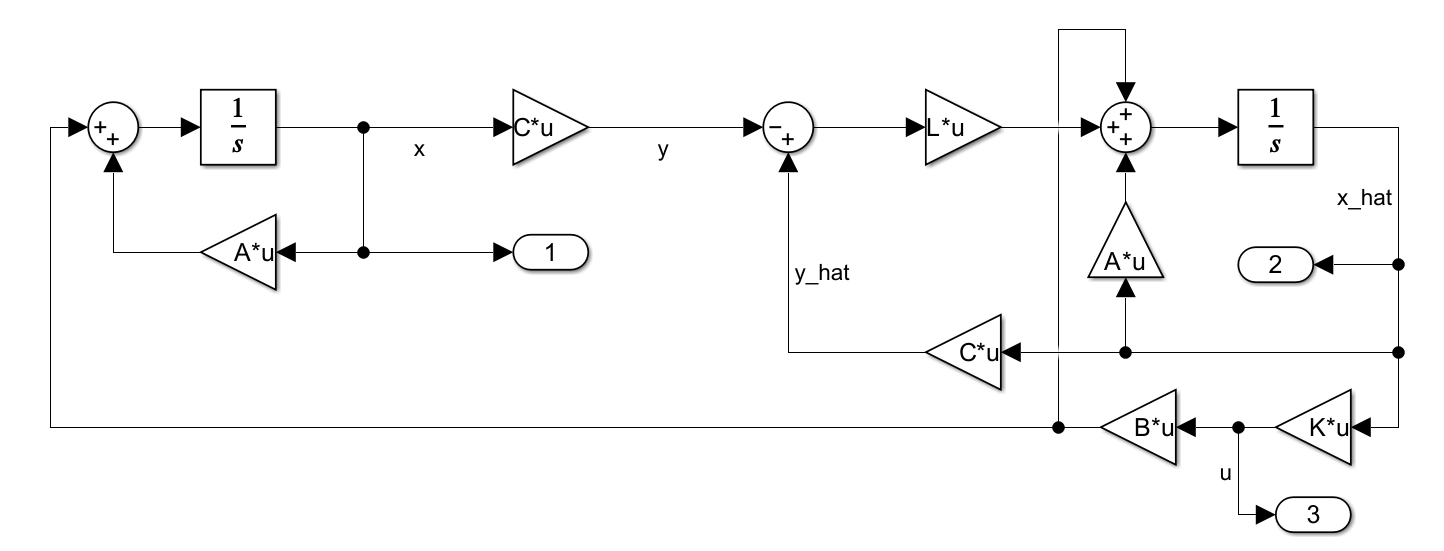
\includegraphics[width=\textwidth]{figs/task2_slx.png}
    \label{fig:sys2}
\end{figure}

Зададимся парой значений $\alpha$: $\alpha_1=10$ и $\alpha_2=2$. Для
дальнейшего исследования зададимся тремя наборами степеней усточивости:
\begin{enumerate}
    \item $\alpha_K=\alpha_L=\alpha_1$ (наблюдатель и регулятор имеют сопоставимые значения);
    \item $\alpha_K=\alpha_1>\alpha_L=\alpha_2$ (регулятор «сильнее»);
    \item $\alpha_K=\alpha_2<\alpha_L=\alpha_1$ (наблюдатель «сильнее»).
\end{enumerate}


\subsection{Первый набор степеней устойчивости}

\subsubsection{Синтез регулятора}

Сначала найдем регулятор со степенью устойчивости $\alpha_K=10$, будем пользоваться
матричным неранством типа Ляпунова с минимизацией управления аналогично \autoref{sec:lyapexp}. 
Используя CVX, получаем
\begin{equation}
    K=\begin{bmatrix}
        213.8675&	156.8793&	-271.5316&	99.1861
    \end{bmatrix},
    \label{eq:K10}
\end{equation}
посмотрим на спектр замкнутой системы
\begin{equation*}
    \sigma(A+BK)=\{-10.0105 \pm 24.5243i,\ -10.8927 \pm 0.5692i \},
\end{equation*}
как видно, система стала устойчивой с желаемой степенью устойчивости и 
минимизированным управлением, хотя степень устойчивости не получилась минимально
возможная, CVX по какой-то причине провалил оптимизацию.


\subsubsection{Синтез наблюдателя}

Теперь найдем матрицу для наблюдателя со степенью сходимости $\alpha_L=10$. 
Для начала нужно ``усечь'' систему, чтобы избавится от ненаблюдаемого собственного
числа. Жорданова форма системы выглядит следующим образом
\begin{equation*}
    A_J=\begin{bmatrix}
        16 & 0  & 0  & 0  \\
         0 & 12 & 0  & 0  \\
         0 & 0  & -12 & 0 \\
         0 & 0  & 0  & 4
    \end{bmatrix},\quad
    C_J=\begin{bmatrix}
        0 & 0 & 0 & 4 \\
        4 & 8 & 0 & 0
    \end{bmatrix},\quad
    P=\begin{bmatrix}
        -1 &  1 & -1 &  1 \\
         1 &  1 & -1 & -1 \\
         1 & -1 & -1 &  1 \\
         1 &  1 &  1 &  1
    \end{bmatrix},
\end{equation*}
где $P$ - матрица перехода. Воспользуемся матричным неравенством типа
Ляпунова для нахождения $L$
\begin{equation}
    Q\succ0,\quad A^TQ+QA+2\alpha Q+C^TY^T+YC\prec0,\quad Q\succ0,\quad L=Q^{-1}Y,
    \label{eq:lyap2}
\end{equation}
и дополнительными матричными неравенствами для минимизации управления
\begin{equation}
    \begin{bmatrix}
        Q&e_0\\
        e_0^T&1
    \end{bmatrix}\succ0,\quad
    \begin{bmatrix}
        Q&Y\\
        Y^T&\gamma I
    \end{bmatrix}\succ0,
    \label{eq:lyap2min}
\end{equation}
с данными неравенствами нужно минимизировать $\gamma$, за $e_0$ возьмем $\begin{bmatrix}
    10&10&10
\end{bmatrix}^T$, пару раз запустив CVX, обраружил, что имеенно данная начальная ошибка
лучше всего прижимает спект ошибки наблюдателя к желаемому. Запустив CVX для неравенств
\ref{eq:lyap2}, \ref{eq:lyap2min} на ``урезанной'' системе получим
\begin{equation*}
    L_j=\begin{bmatrix}
        -1.5231 & -62.8207 \\
         0.9779 &  25.4104 \\
        -3.6795 &  -0.0001
    \end{bmatrix},
\end{equation*}
дополним нулями
\begin{equation*}
    L_J=\begin{bmatrix}
        -1.5231 & -62.8207 \\
         0.9779 &  25.4104 \\
         0&0\\
        -3.6795 &  -0.0001
    \end{bmatrix},
\end{equation*}
и вернем в изначальный базис
\begin{equation}
    L=PL_J=\begin{bmatrix}
        -1.1785 &  88.2310 \\
         3.1342 & -37.4103 \\
        -6.1805 & -88.2312 \\
        -4.2247 & -37.4104
    \end{bmatrix}.
    \label{eq:L10}
\end{equation}
Проверим результат посмотрев на спектр ошибки наблюдателя
\begin{equation*}
    \sigma(A+LC)=\{-10.0000 \pm 18.1421i,\ -10.7179,\ -12 \},
\end{equation*}
как видно, управление было минимизировано, и требуемая степень сходимости достигнута.

\subsubsection{Моделирование}

Выполним компьютерное моделирование с начальными условиями системы
$x(0)=\begin{bmatrix}
    1&1&1&1
\end{bmatrix}^T$ и наблюдателя $\hat x(0)=\begin{bmatrix}
    0&0&0&0
\end{bmatrix}^T.$ Построим графики (см \autoref{fig:21})
формируемого регулятором управления $u(t)$, сравнительные графики $x(t)$ и
$\hat x(t)$, а также график ошибки наблюдателя $e(t) = x(t) -\hat x(t).$

\begin{figure}[H]
    \centering
    \caption{Моделирование системы \eqref{eq:sys2} с регулятором вида $u=K\hat x$
    и наблюдателем состояния $\dot{\hat x}=A\hat x+Bu+L(C\hat x-y)$ при $\alpha_K=\alpha_L$}
    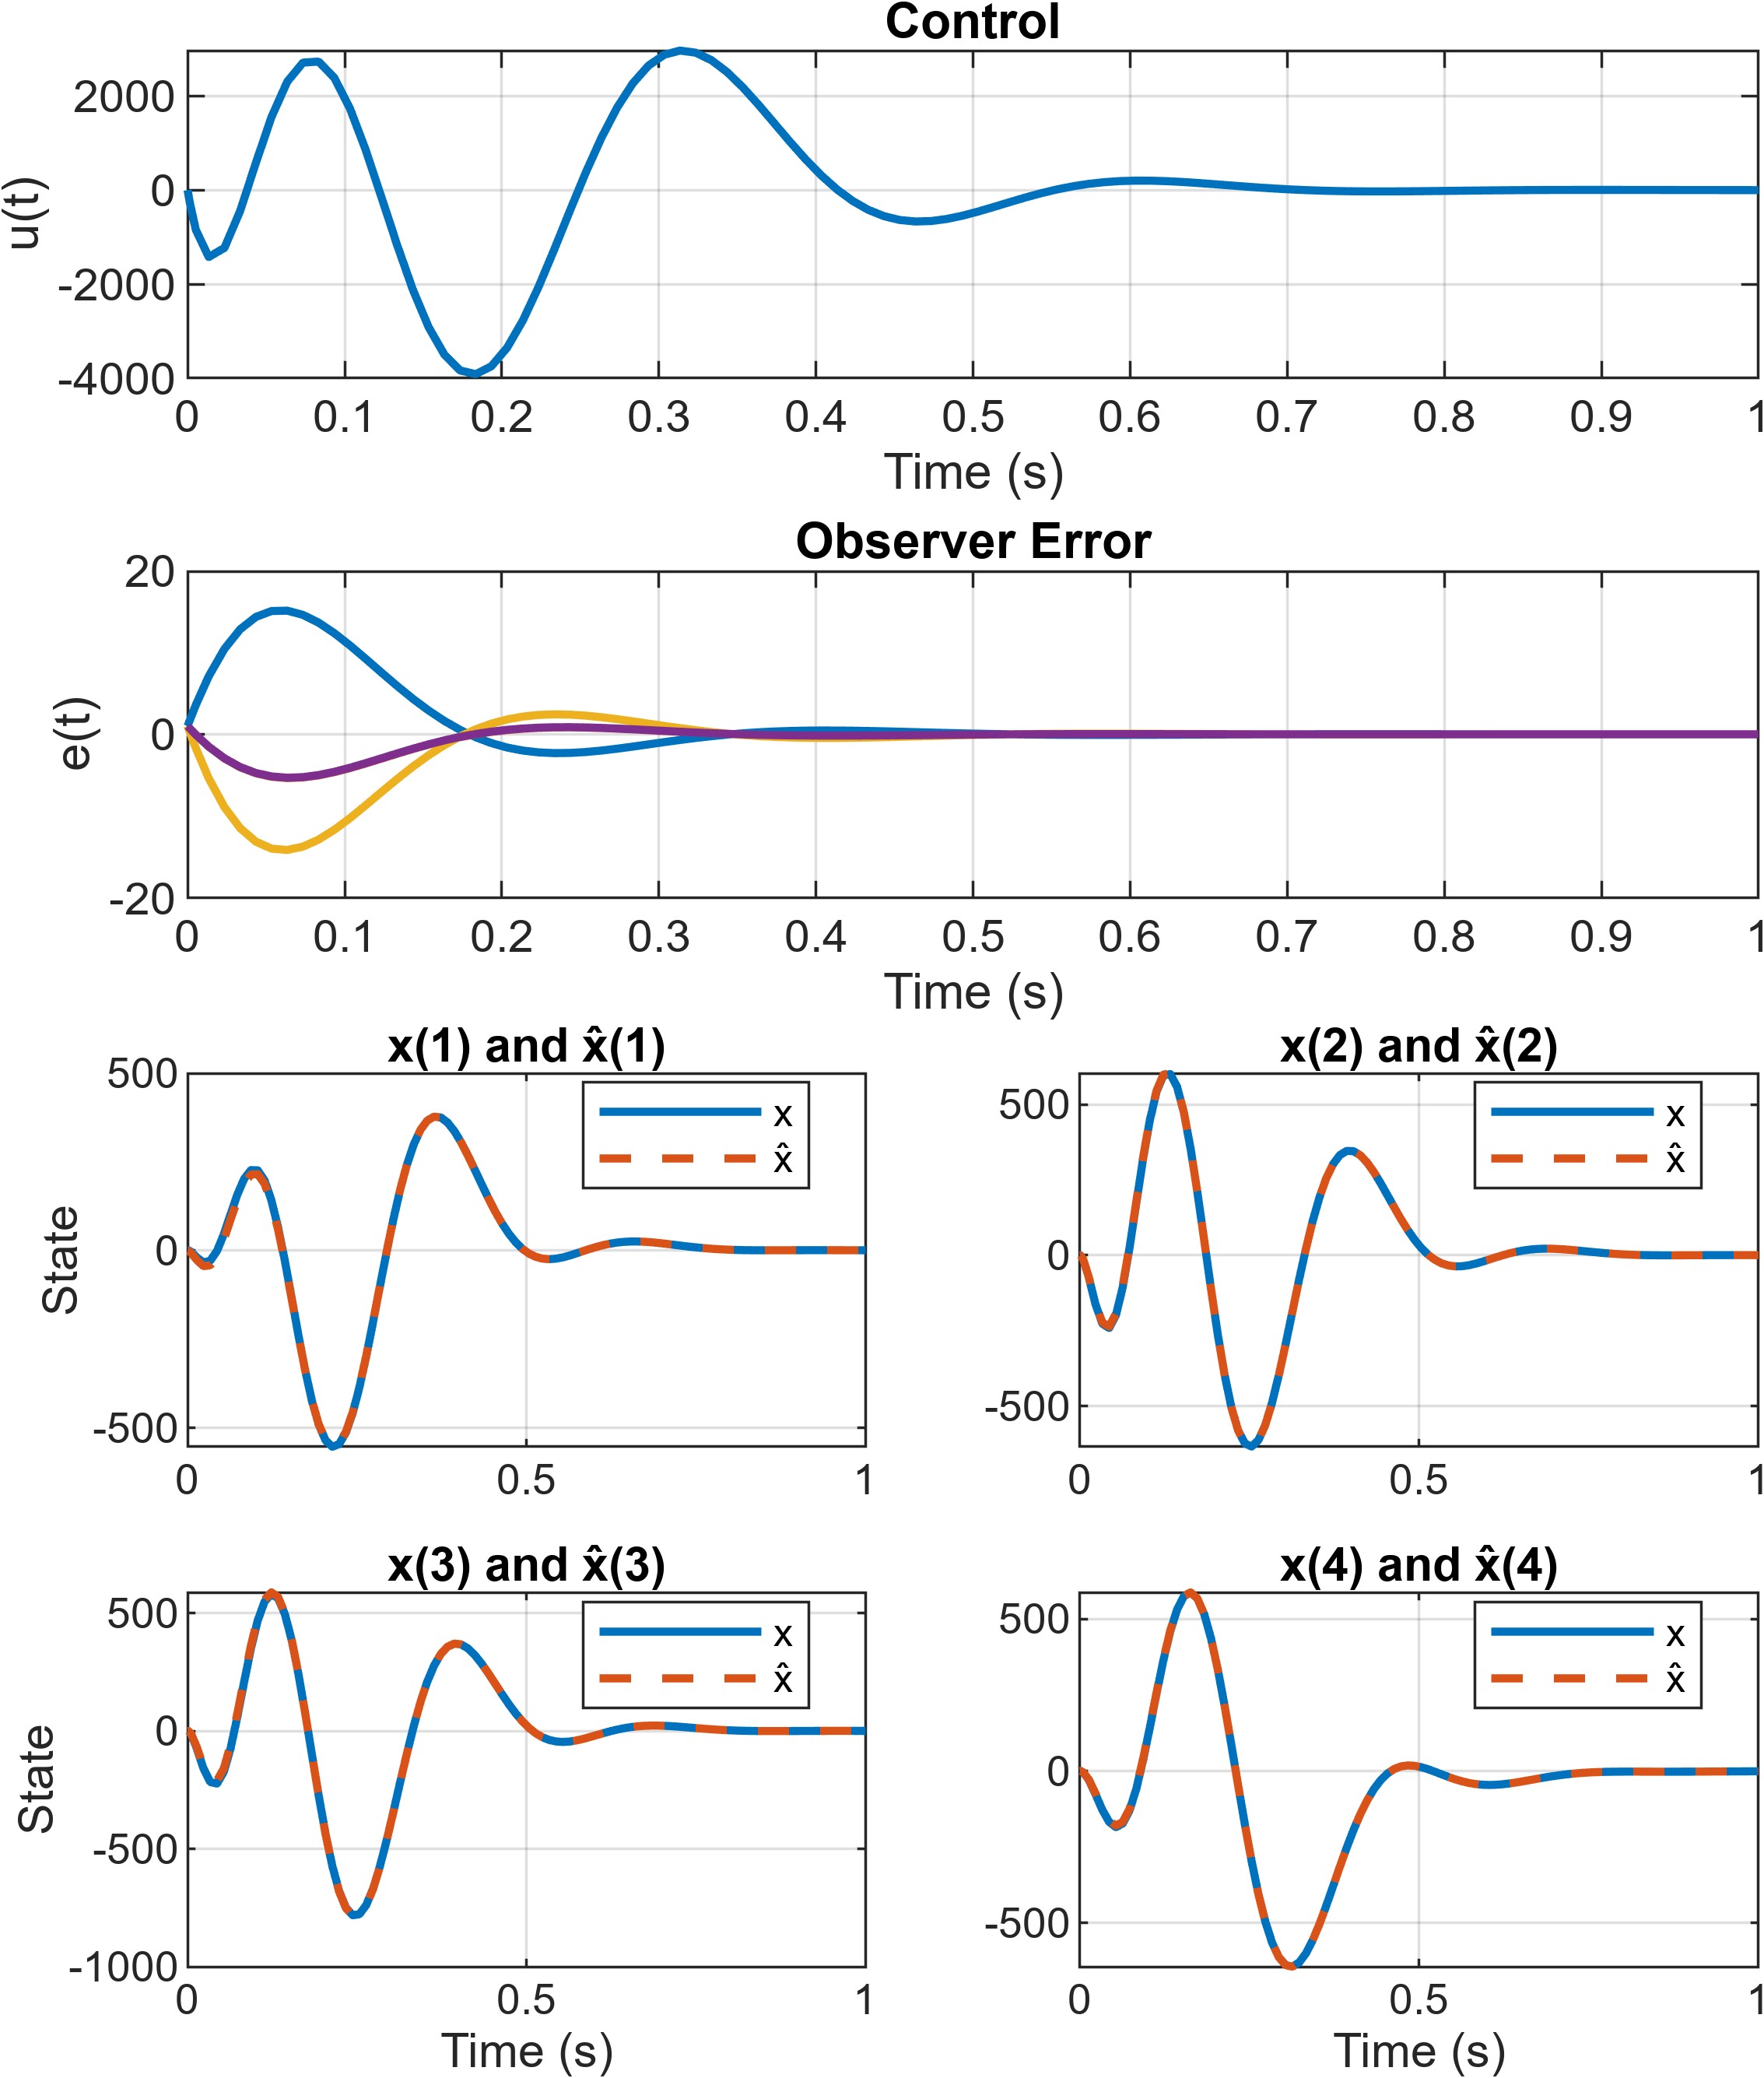
\includegraphics[width=\linewidth]{figs/task2_1.png}
    \label{fig:21}
\end{figure}



\subsection{Второй набор степеней устойчивости}


Рассмотрим случай, когда регулятор ``сильнее'' наблюдателя, регулятор будем
использовать из предыдущего раздела \autoref{eq:K10}.


\subsubsection{Синтез наблюдателя}

Аналогично предыдущему разделу найдем матрицу для наблюдателя 
со степенью сходимости $\alpha_L=2$. 
Запустив CVX для неравенств на ``урезанной'' системе получим
\begin{equation*}
    L_j=\begin{bmatrix}
        -1.9997&	-29.8223\\
        1.1213&	10.9112\\
        -1.5975&	0.0000
    \end{bmatrix},
\end{equation*}
дополним нулями и вернем в изначальный базис
\begin{equation*}
    L=\begin{bmatrix}
        1.5234&	40.7335\\
        0.7192&	-18.9112\\
        -4.7185&	-40.7335\\
        -2.4759&	-18.9112
    \end{bmatrix}.
\end{equation*}
Проверим результат посмотрев на спектр ошибки наблюдателя
\begin{equation*}
    \sigma(A+LC)=\{-2 \pm12.3757i,\ -12,\ -2.3902 \},
\end{equation*}
как видно, управление было минимизировано, и требуемая степень сходимости достигнута.

\subsubsection{Моделирование}

Выполним компьютерное моделирование с начальными условиями системы
$x(0)=\begin{bmatrix}
    1&1&1&1
\end{bmatrix}^T$ и наблюдателя $\hat x(0)=\begin{bmatrix}
    0&0&0&0
\end{bmatrix}^T.$ Построим графики (см \autoref{fig:22})
формируемого регулятором управления $u(t)$, сравнительные графики $x(t)$ и
$\hat x(t)$, а также график ошибки наблюдателя $e(t) = x(t) -\hat x(t).$

\begin{figure}[H]
    \centering
    \caption{Моделирование системы \eqref{eq:sys2} с регулятором вида $u=K\hat x$
    и наблюдателем состояния $\dot{\hat x}=A\hat x+Bu+L(C\hat x-y)$ при $\alpha_K>\alpha_L$}
    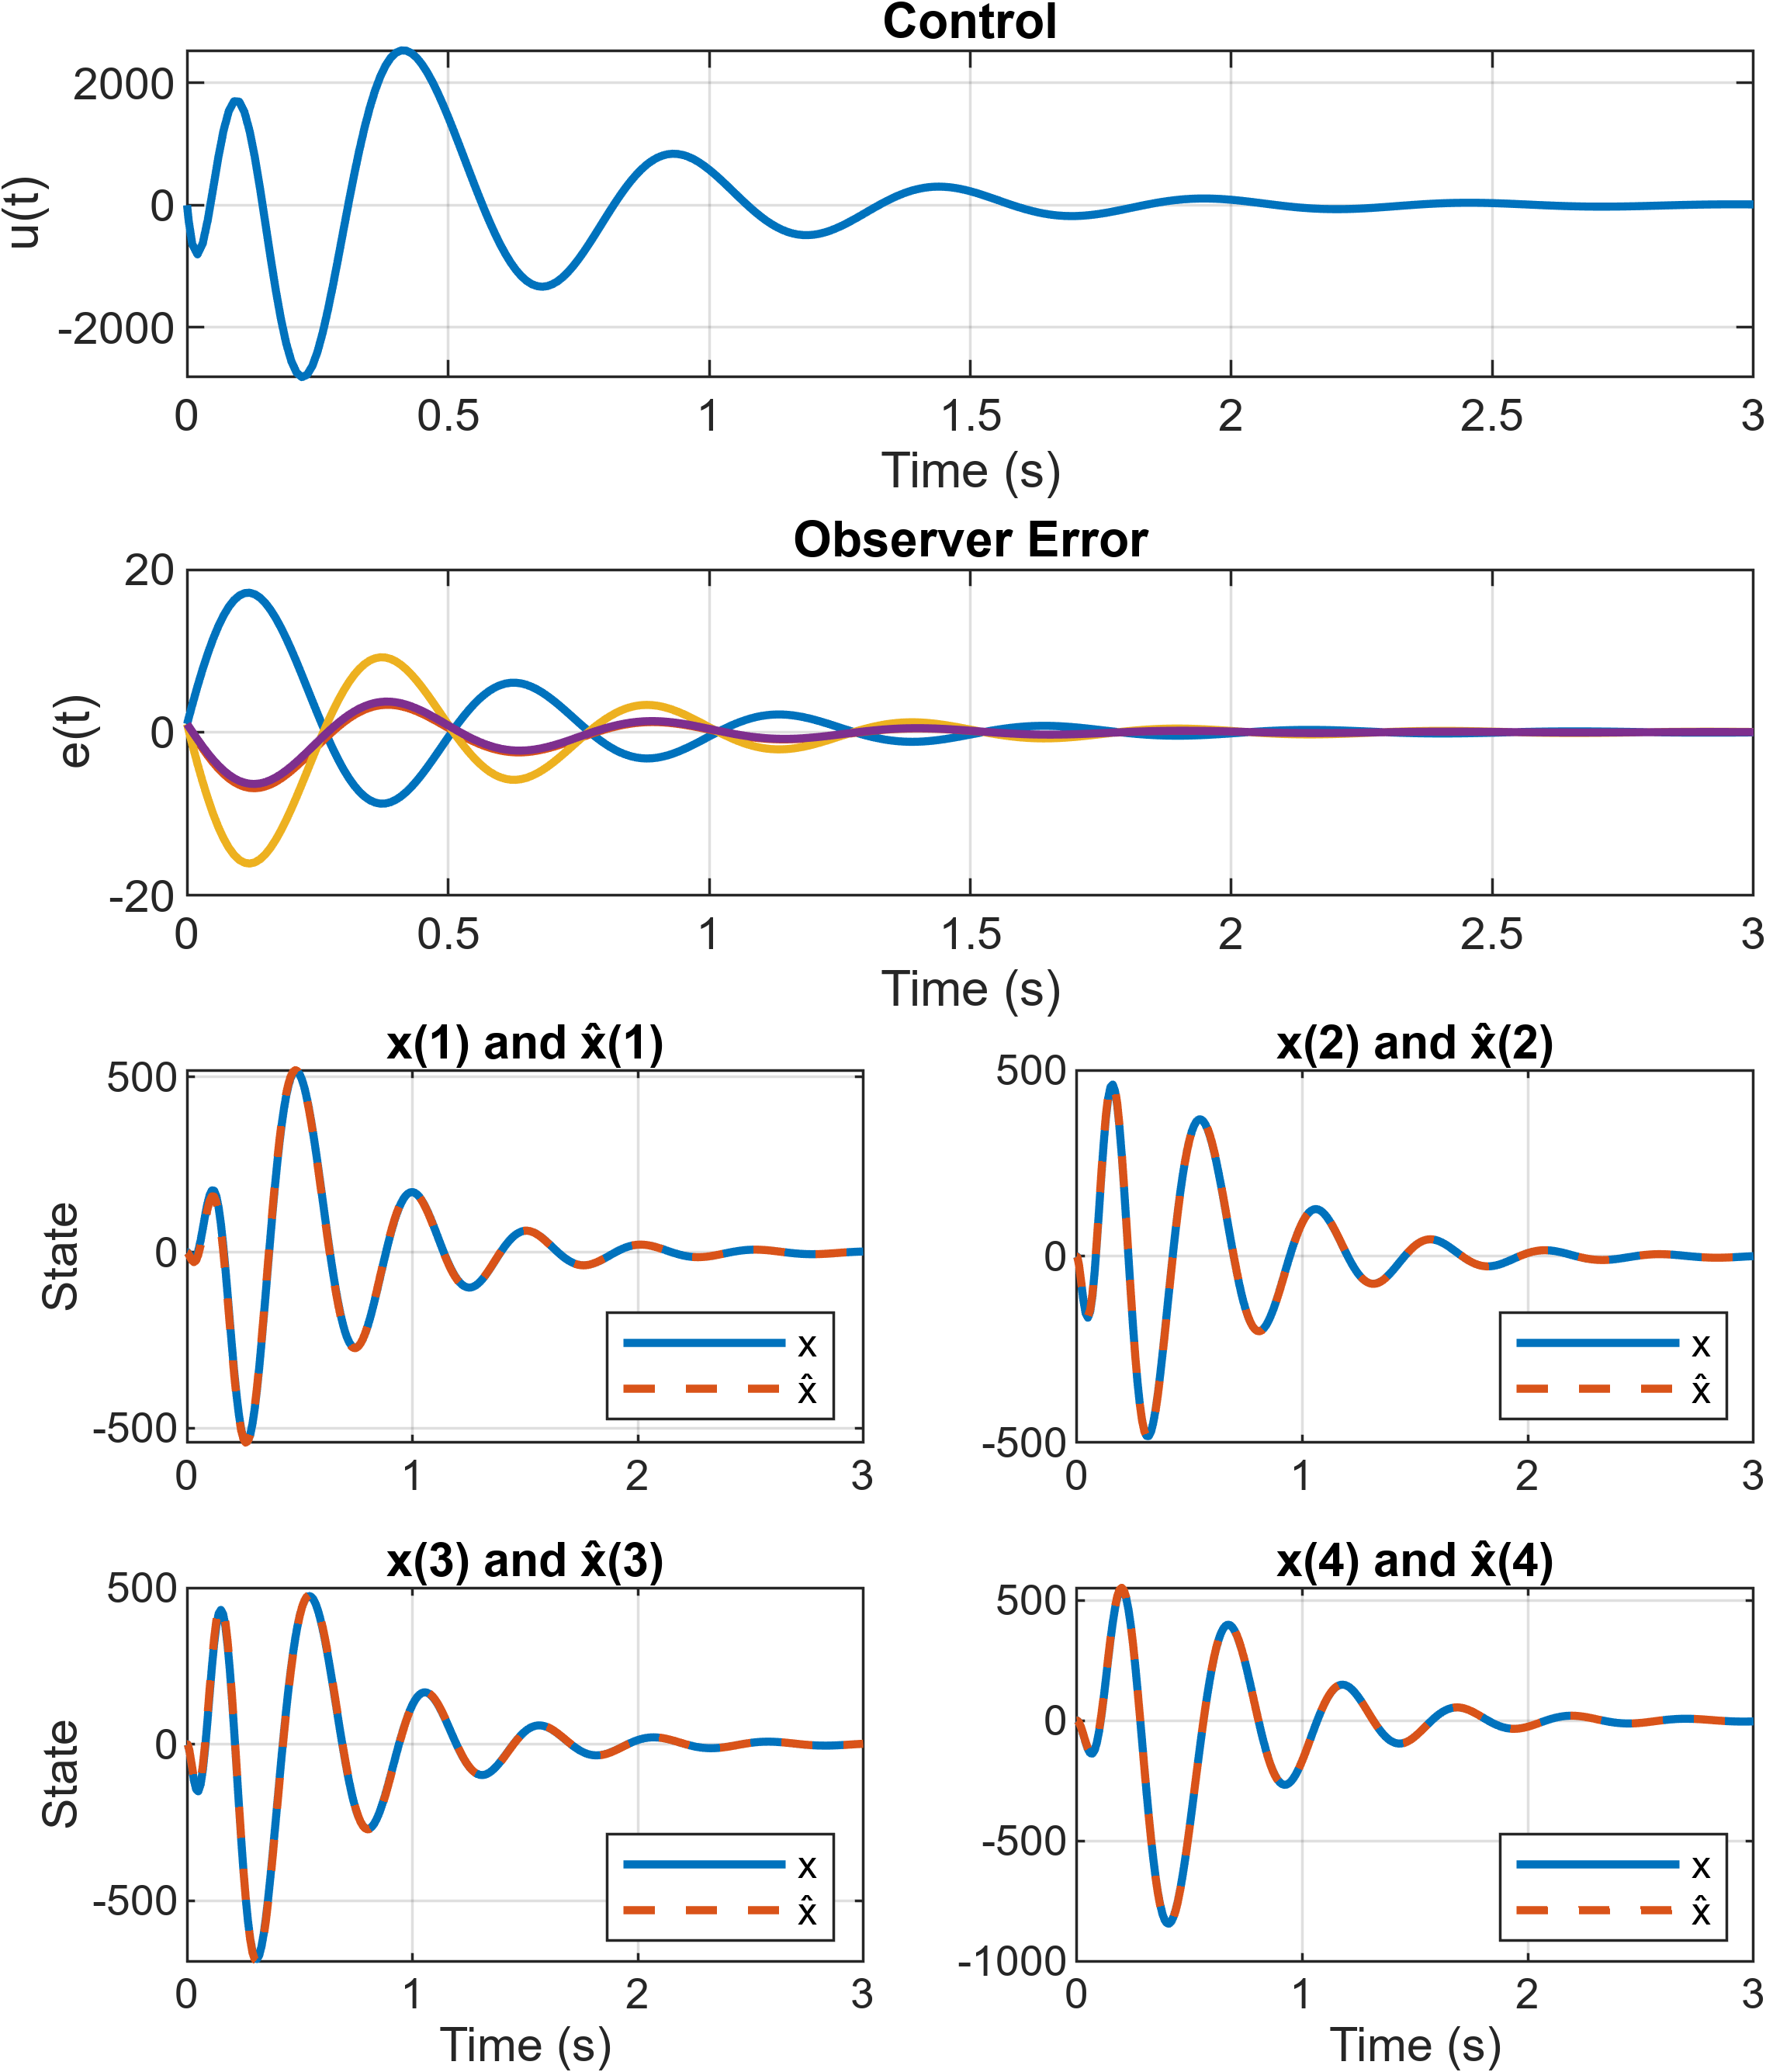
\includegraphics[width=\linewidth]{figs/task2_2.png}
    \label{fig:22}
\end{figure}


\newpage
\subsection{Третий набор степеней устойчивости}


Рассмотрим случай, когда наблюдатель ``сильнее'' регулятора, наблюдатель будем
использовать из \autoref{eq:L10}.


\subsubsection{Синтез регулятора}

Аналогично \autoref{sec:lyapexp} найдем регулятор со степенью устойчивости $\alpha_K=2$
с помощью матричного неранства типа Ляпунова с минимизацией управления. 
Используя CVX, получаем
\begin{equation*}
    K=\begin{bmatrix}
        49.7464&	25.9350&	-55.5580&	20.1232
    \end{bmatrix},
\end{equation*}
посмотрим на спектр замкнутой системы
\begin{equation*}
    \sigma(A+BK)=\{-2.0004 \pm12.2470i,\ -11.9975,\ -2.0004 \},
\end{equation*}
как видно, система стала устойчивой с желаемой степенью устойчивости и 
минимизированным управлением, но, хотя система полностью управляемая, 
CVX по какой-то причине не до оптимизировал третье собственное число, выдав
такой статус решения Inaccurate/Solved.


\subsubsection{Моделирование}

Выполним компьютерное моделирование с начальными условиями системы
$x(0)=\begin{bmatrix}
    1&1&1&1
\end{bmatrix}^T$ и наблюдателя $\hat x(0)=\begin{bmatrix}
    0&0&0&0
\end{bmatrix}^T.$ Построим графики (см \autoref{fig:23})
формируемого регулятором управления $u(t)$, сравнительные графики $x(t)$ и
$\hat x(t)$, а также график ошибки наблюдателя $e(t) = x(t) -\hat x(t).$

\begin{figure}[H]
    \centering
    \caption{Моделирование системы \eqref{eq:sys2} с регулятором вида $u=K\hat x$
    и наблюдателем состояния $\dot{\hat x}=A\hat x+Bu+L(C\hat x-y)$ при $\alpha_K<\alpha_L$}
    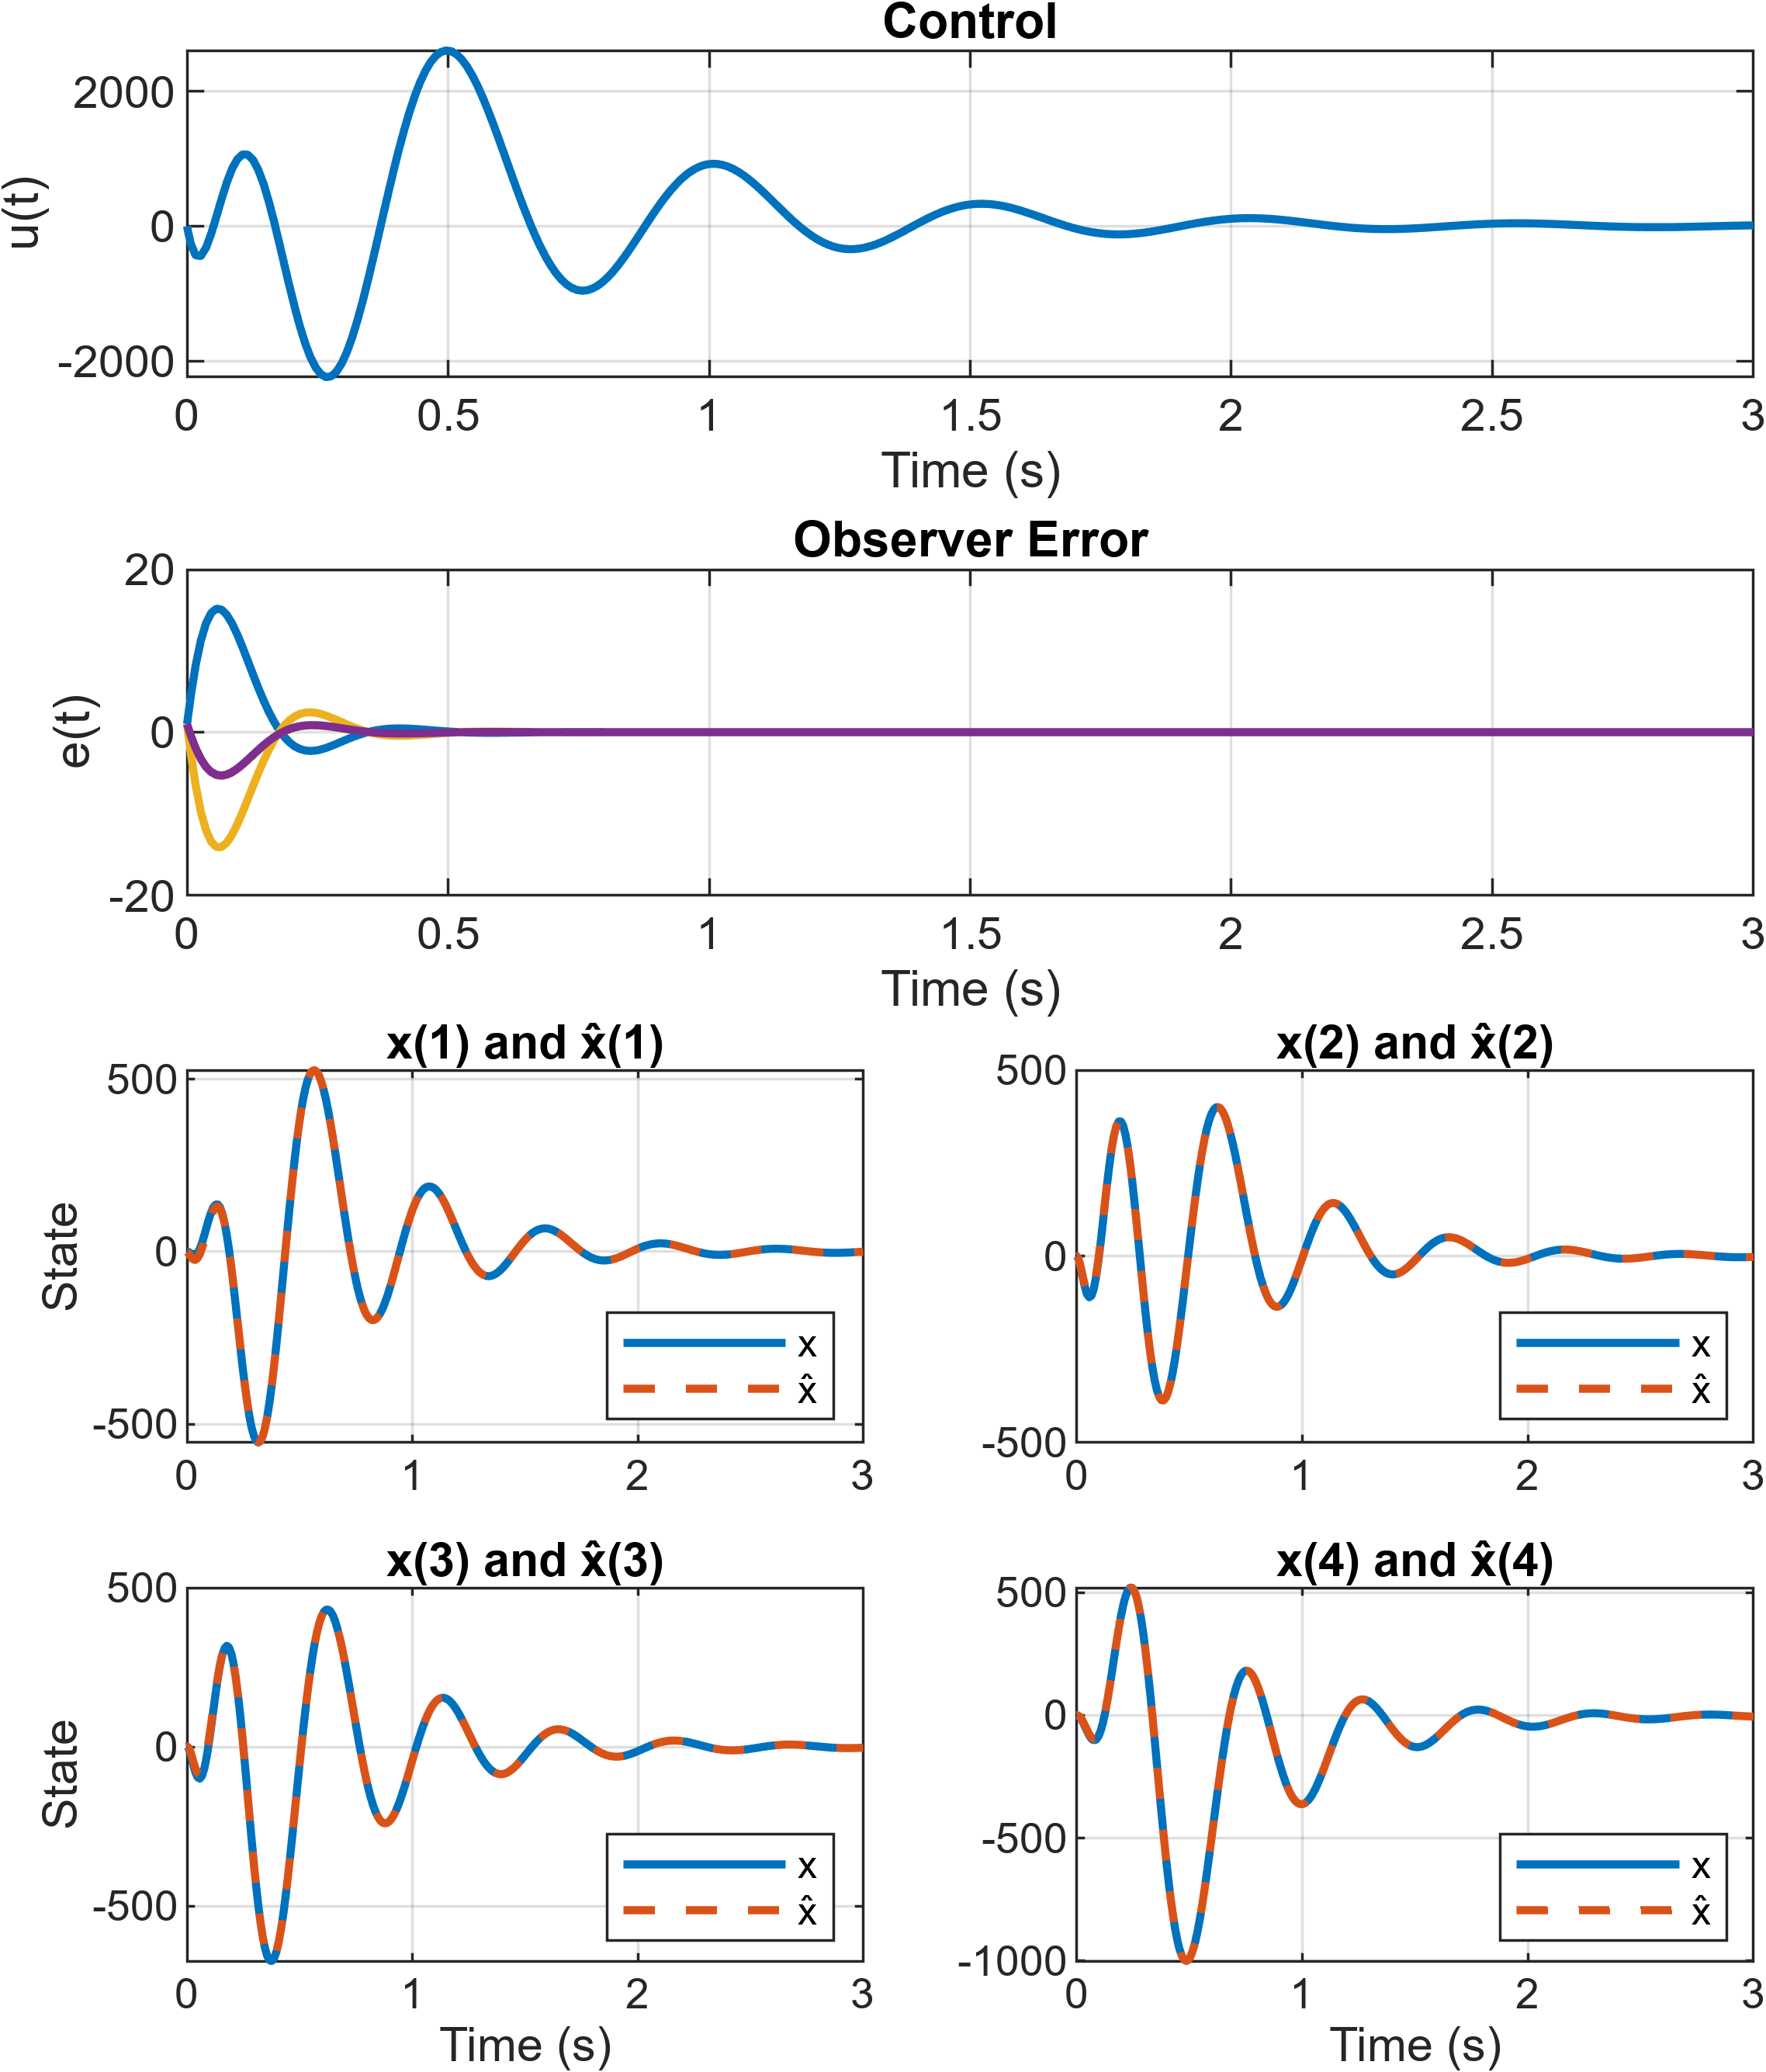
\includegraphics[width=\linewidth]{figs/task2_3.png}
    \label{fig:23}
\end{figure}


\subsection{Выводы}

Были рассмотрены три различных набора степеней устойчивости регулятора $\alpha_K$ 
и степени сходимости наблюдателя $\alpha_L$. 
\begin{itemize}
    \item В случае, когда $\alpha_K = \alpha_L = 10$ ошибка наблюдателя быстро сходится к нулю,
    как и состояние системы. 
    \item Когда $\alpha_K=10 > \alpha_L=2$ наблюдатель сходился заметно дольше, и так как
    регулятор зависит от оценки состояния системы, состояние системы пришло в ноль только
    после схождения ошибки наблюдателя.
    \item В случае $\alpha_K=2 < \alpha_L=10$, ошибка наблюдателя быстро пришла в ноль, но
    состояние системы еще должгое колебалось из-за ``слабого'' регулятора.
\end{itemize}
Таким образом, при зависимости регулятора от оценки состояния системы, скорость
сходимости состояния зависит от скорости сходимости наблюдателя, состояние не может
прийти в ноль выстрее невязки наблюдателя.



\section{Регулятор с качественной экспоненциальной устойчивостью}

\subsection{Анализ системы}

Рассмотрим систему
\begin{equation}
    \dot x=Ax+Bu,\quad A=\begin{bmatrix}
        3&5&4\\
        -2&-4&-5\\
        2&2&3
    \end{bmatrix},\quad B=\begin{bmatrix}
        2\\-1\\1
    \end{bmatrix}
\end{equation}
из \autoref{sec:anal1}, собственные числа матрицы $A$
\begin{equation*}
    \sigma(A)=\{\ 2\pm i,\ -2\ \}.
\end{equation*}
Ссылаясь на \autoref{sec:anal1}, система не полностью управляема, 
но стабилизируема, так как единственное
неуправляемое собственное число $-2$ отрицательно.

Зададимся параметрами $\beta=-4$ и $r=2$ и четырьмя наборами $Q$ И $R$:
\begin{itemize}
    \item $Q=I,\ R=1$;
    \item $Q=I,\ R=0$;
    \item $Q=0,\ R=1$;
    \item $Q=0,\ R=0$.
\end{itemize}


\subsection{Синтез для первого набора параметров}

Синтезируем регулятор, обеспечивающий качественную экспоненциальную 
устойчивость, с помощью матричного уравнения Риккати:
\begin{equation}
    (A-BK-\beta I)^TP(A-BK-\beta I)-r^2P=-Q,\quad K=-(R+B^TPB)^{-1}B^TP(A-\beta I),
    \label{eq:riccal}
\end{equation}
где $P$ -  искомая симметричная квадратная матрица, $A$, $B$ - матрицы объекта управления,
$Q$, $R$ - симметричные положительно-полуопределенные матрицы. Так как требуется,
что бы пара $(A, B)$ была устойчива, будем искать решение для ``усеченной'' 
системы \eqref{eq:sys1j}. Воспользуемся vpasolve для нахождения матрицы $K_j$ 
при $Q=I$, $R=1$ и,
не с первого раза, получаем
\begin{equation*}
    K_j = \begin{bmatrix}
        0.6538& 2.1135
    \end{bmatrix},
\end{equation*}
дополняем нулями
\begin{equation*}
    K_J = \begin{bmatrix}
        0& 0.6538& 2.1135
    \end{bmatrix},
\end{equation*}
и находим в исходном базисе
\begin{equation*}
    K_1=K_JP^{-1}=\begin{bmatrix}
        -0.6366&	-0.6366&	-9.9318
    \end{bmatrix},
\end{equation*}
матрица $P$ из \autoref{eq:sys1jourdan}.
В подтверждение посмотрим на спектр замкнутой системы
\begin{equation*}
    \sigma(A+BK_1)=\{-3.2842 \pm 1.2648i,\ -2 \},
\end{equation*}
как видно, система стала устойчивой. 


\subsection{Синтез для второго набора параметров}

Аналогично синтезируем регулятор при $Q=I$, $R=0$, получаем
\begin{equation*}
    K_2=\begin{bmatrix}
        -0.5879& -0.5879& -10.7655
    \end{bmatrix}.
\end{equation*}
В подтверждение посмотрим на спектр замкнутой системы
\begin{equation*}
    \sigma(A+BK_2)=\{-2,\ -3.3535,\ -4 \},
\end{equation*}
как видно, система стала устойчивой. 


\subsection{Синтез для третьего набора параметров}

Аналогично синтезируем регулятор при $Q=0$, $R=1$, получаем
\begin{equation*}
    K_3=\begin{bmatrix}
        -1 -1 -11
    \end{bmatrix}.
\end{equation*}
В подтверждение посмотрим на спектр замкнутой системы
\begin{equation*}
    \sigma(A+BK_3)=\{-2,\ -2,\ -6 \},
\end{equation*}
как видно, система стала устойчивой. 


\subsection{Синтез для третьего набора параметров}

Аналогично синтезируем регулятор при $Q=0$, $R=0$, получаем
\begin{equation*}
    K_4=\begin{bmatrix}
        -1.2761& -1.2761& -8.9303   
    \end{bmatrix}.
\end{equation*}
В подтверждение посмотрим на спектр замкнутой системы
\begin{equation*}
    \sigma(A+BK_4)=\{-2.2065,\ -4,\ -2\},
\end{equation*}
как видно, система стала устойчивой. 


\subsection{Визуализация спектров}

Выведим спектры на комплексную
плоскость, проверив, находятся ли они в пределах
круга с центром в точке $(\beta, 0)$ и радиусом $r$ в подтверждение 
корректности синтеза регуляторов. Как можно увидеть на \autoref{fig:riccati1},
все собственные числа находятся в пределах круга, значит регуляторы
синтезированы правильно.

\begin{figure}[H]
    \centering
    \caption{Спектры замкнутых систем \eqref{eq:sys1} с регулятором с 
    качественной экспоненциальной устойчивостью}
    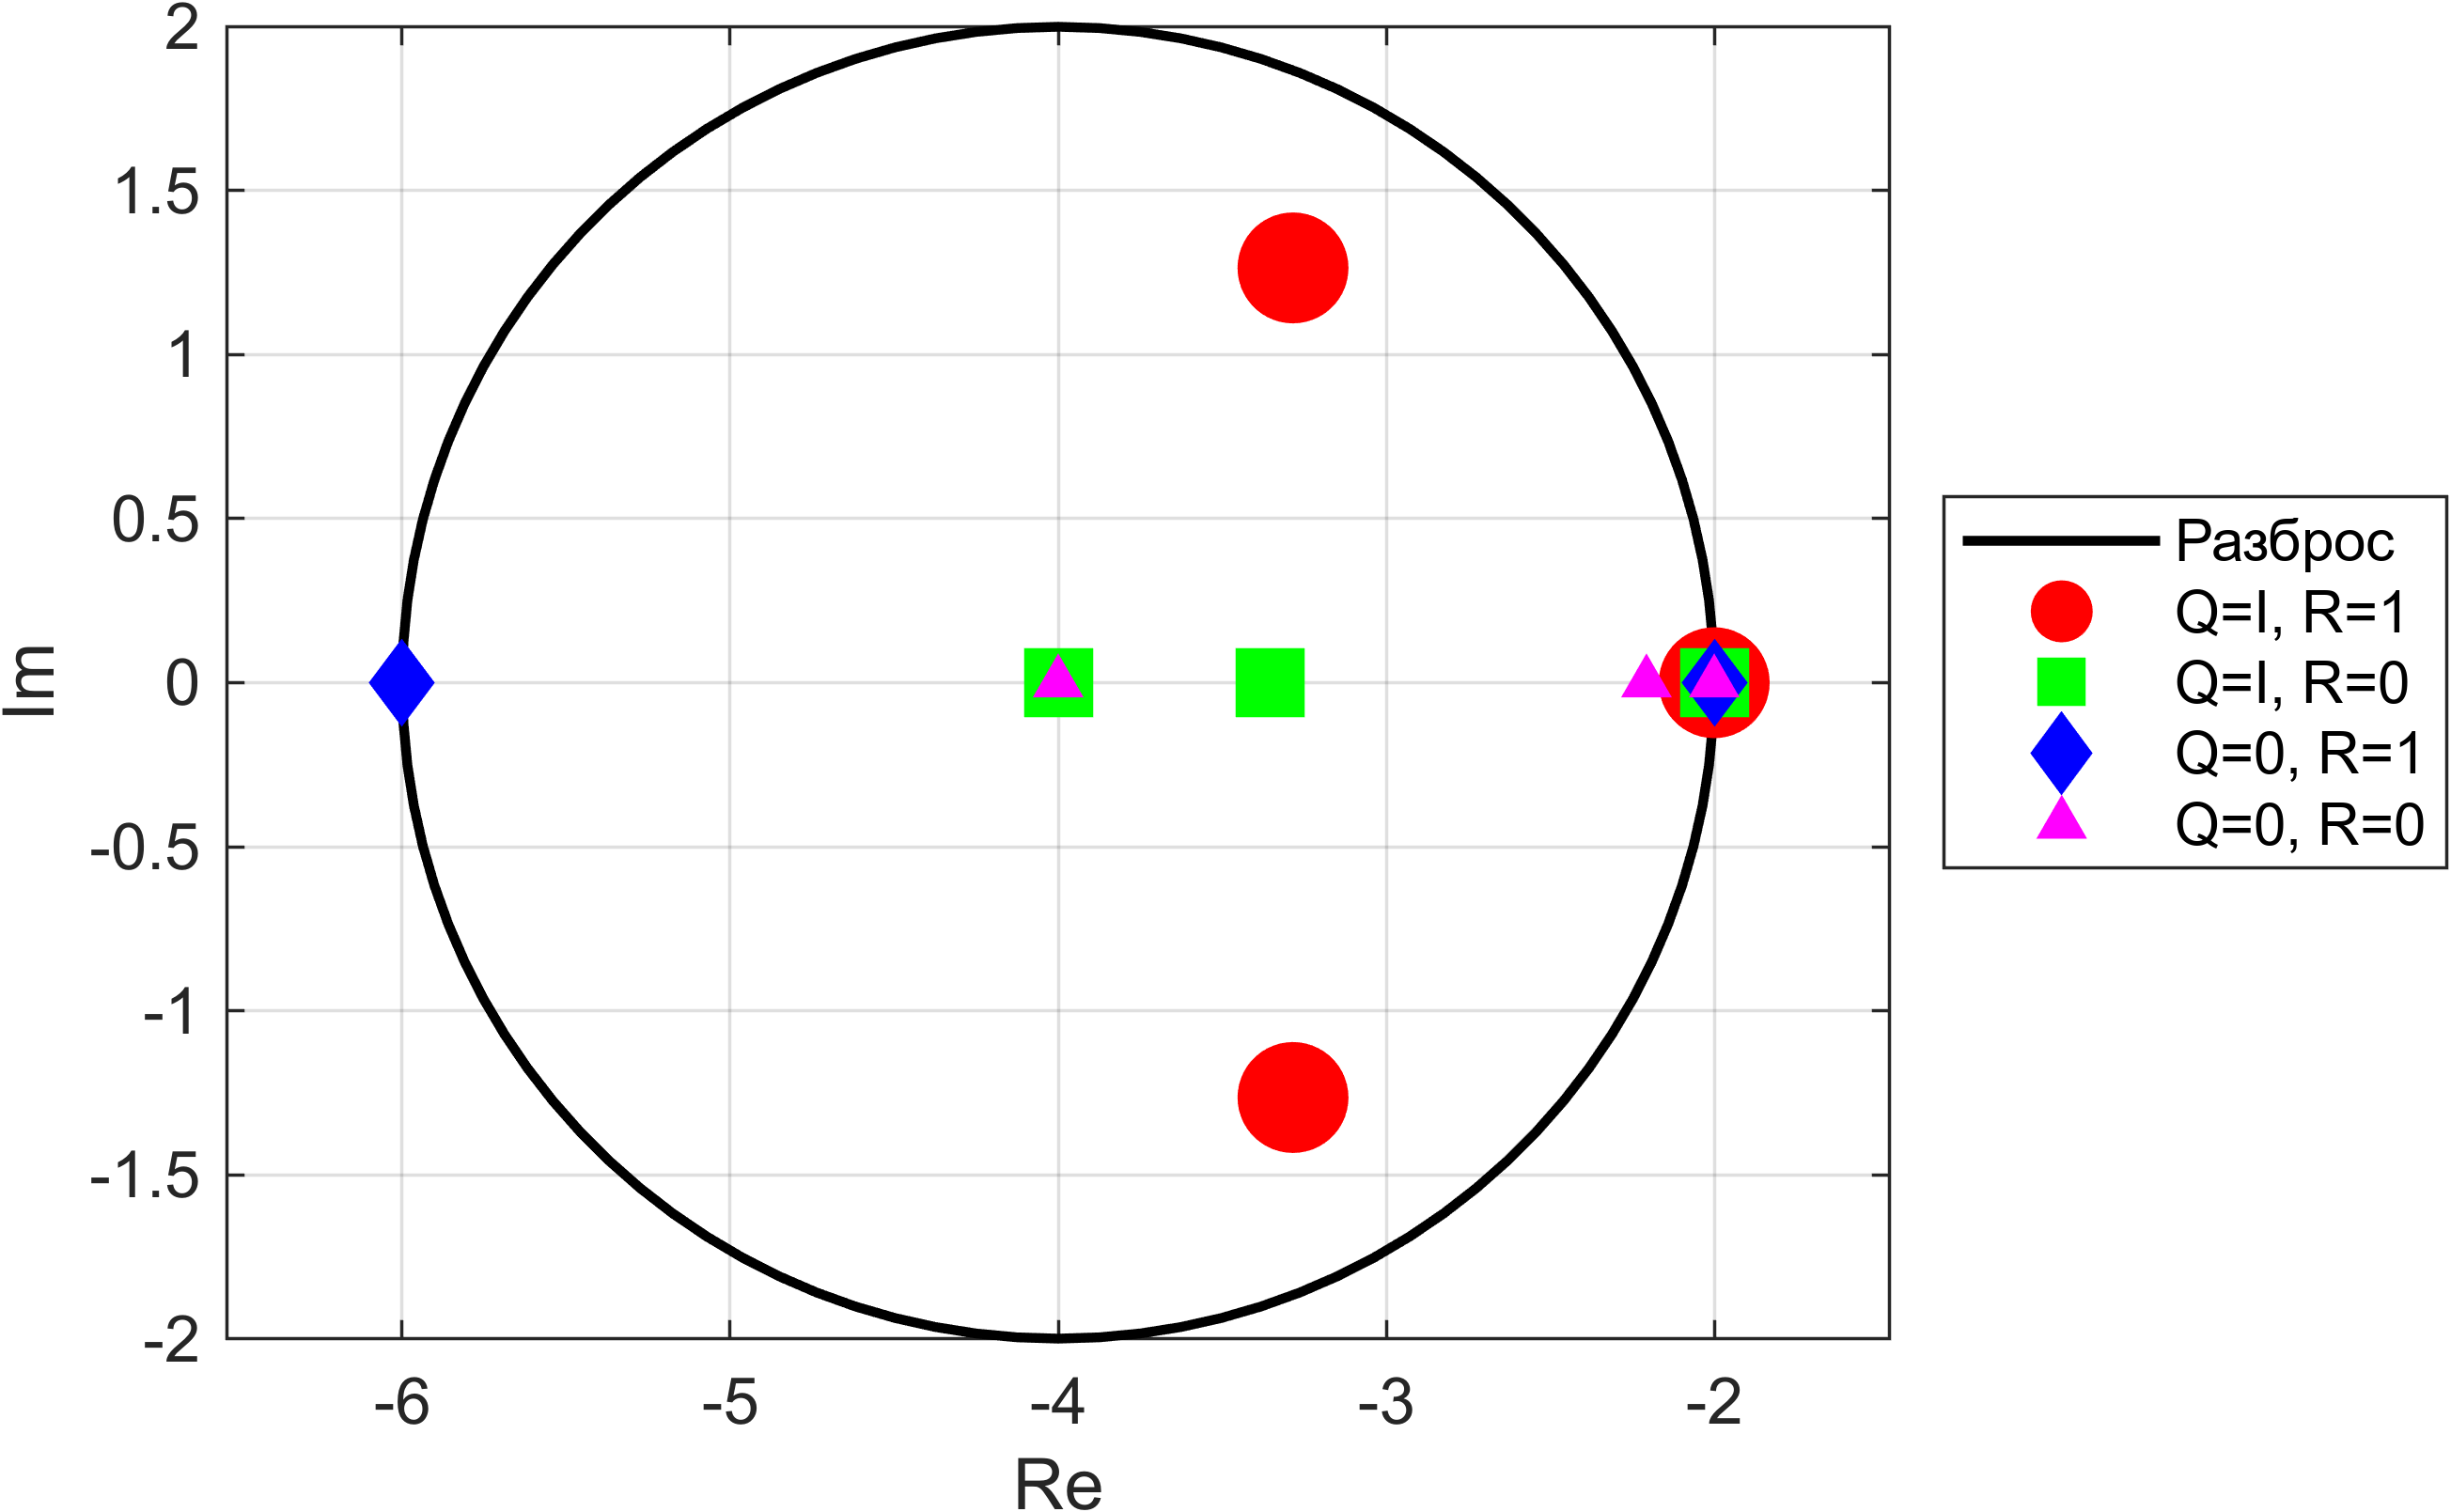
\includegraphics[width=\linewidth]{figs/task3.png}
    \label{fig:riccati1}
\end{figure}


\subsection{Моделирование}

Выполним компьютерное моделирование замкнутой системы и построим
графики формируемого регулятором управления $u(t)$ и вектора состояния
замкнутой системы $x(t)$ при начальных условиях $x(0) =\begin{bmatrix}
    1&1&1
\end{bmatrix}^T$. Результат можно увидеть на \autoref{fig:riccati2},
поведение системы очень слабо изменяется при разных наборах
$Q$ и $R$.


\subsection{Выводы}

Были синтезированы регуляторы с качественной экспоненциальной устойчивостью для 
нулевых и единичных наборов параметров $Q$ и $R$ при $\beta=-4$ и $r=2$. Все 
регуляторы обеспечили устойчивость 
системы, а спектры замкнутых систем находились в пределах заданного круга, что 
подтверждает корректность синтеза. Моделирование показало схожее поведение системы 
при разных параметрах, что указывает на слабую зависимость динамики от выбора 
нулевых или единичных $Q$ и $R$.


\begin{figure}[H]
    \centering
    \caption{Моделирование замкнутой системы \eqref{eq:sys1} с регулятором с
    качественной экспоненциальной устойчивостью}
    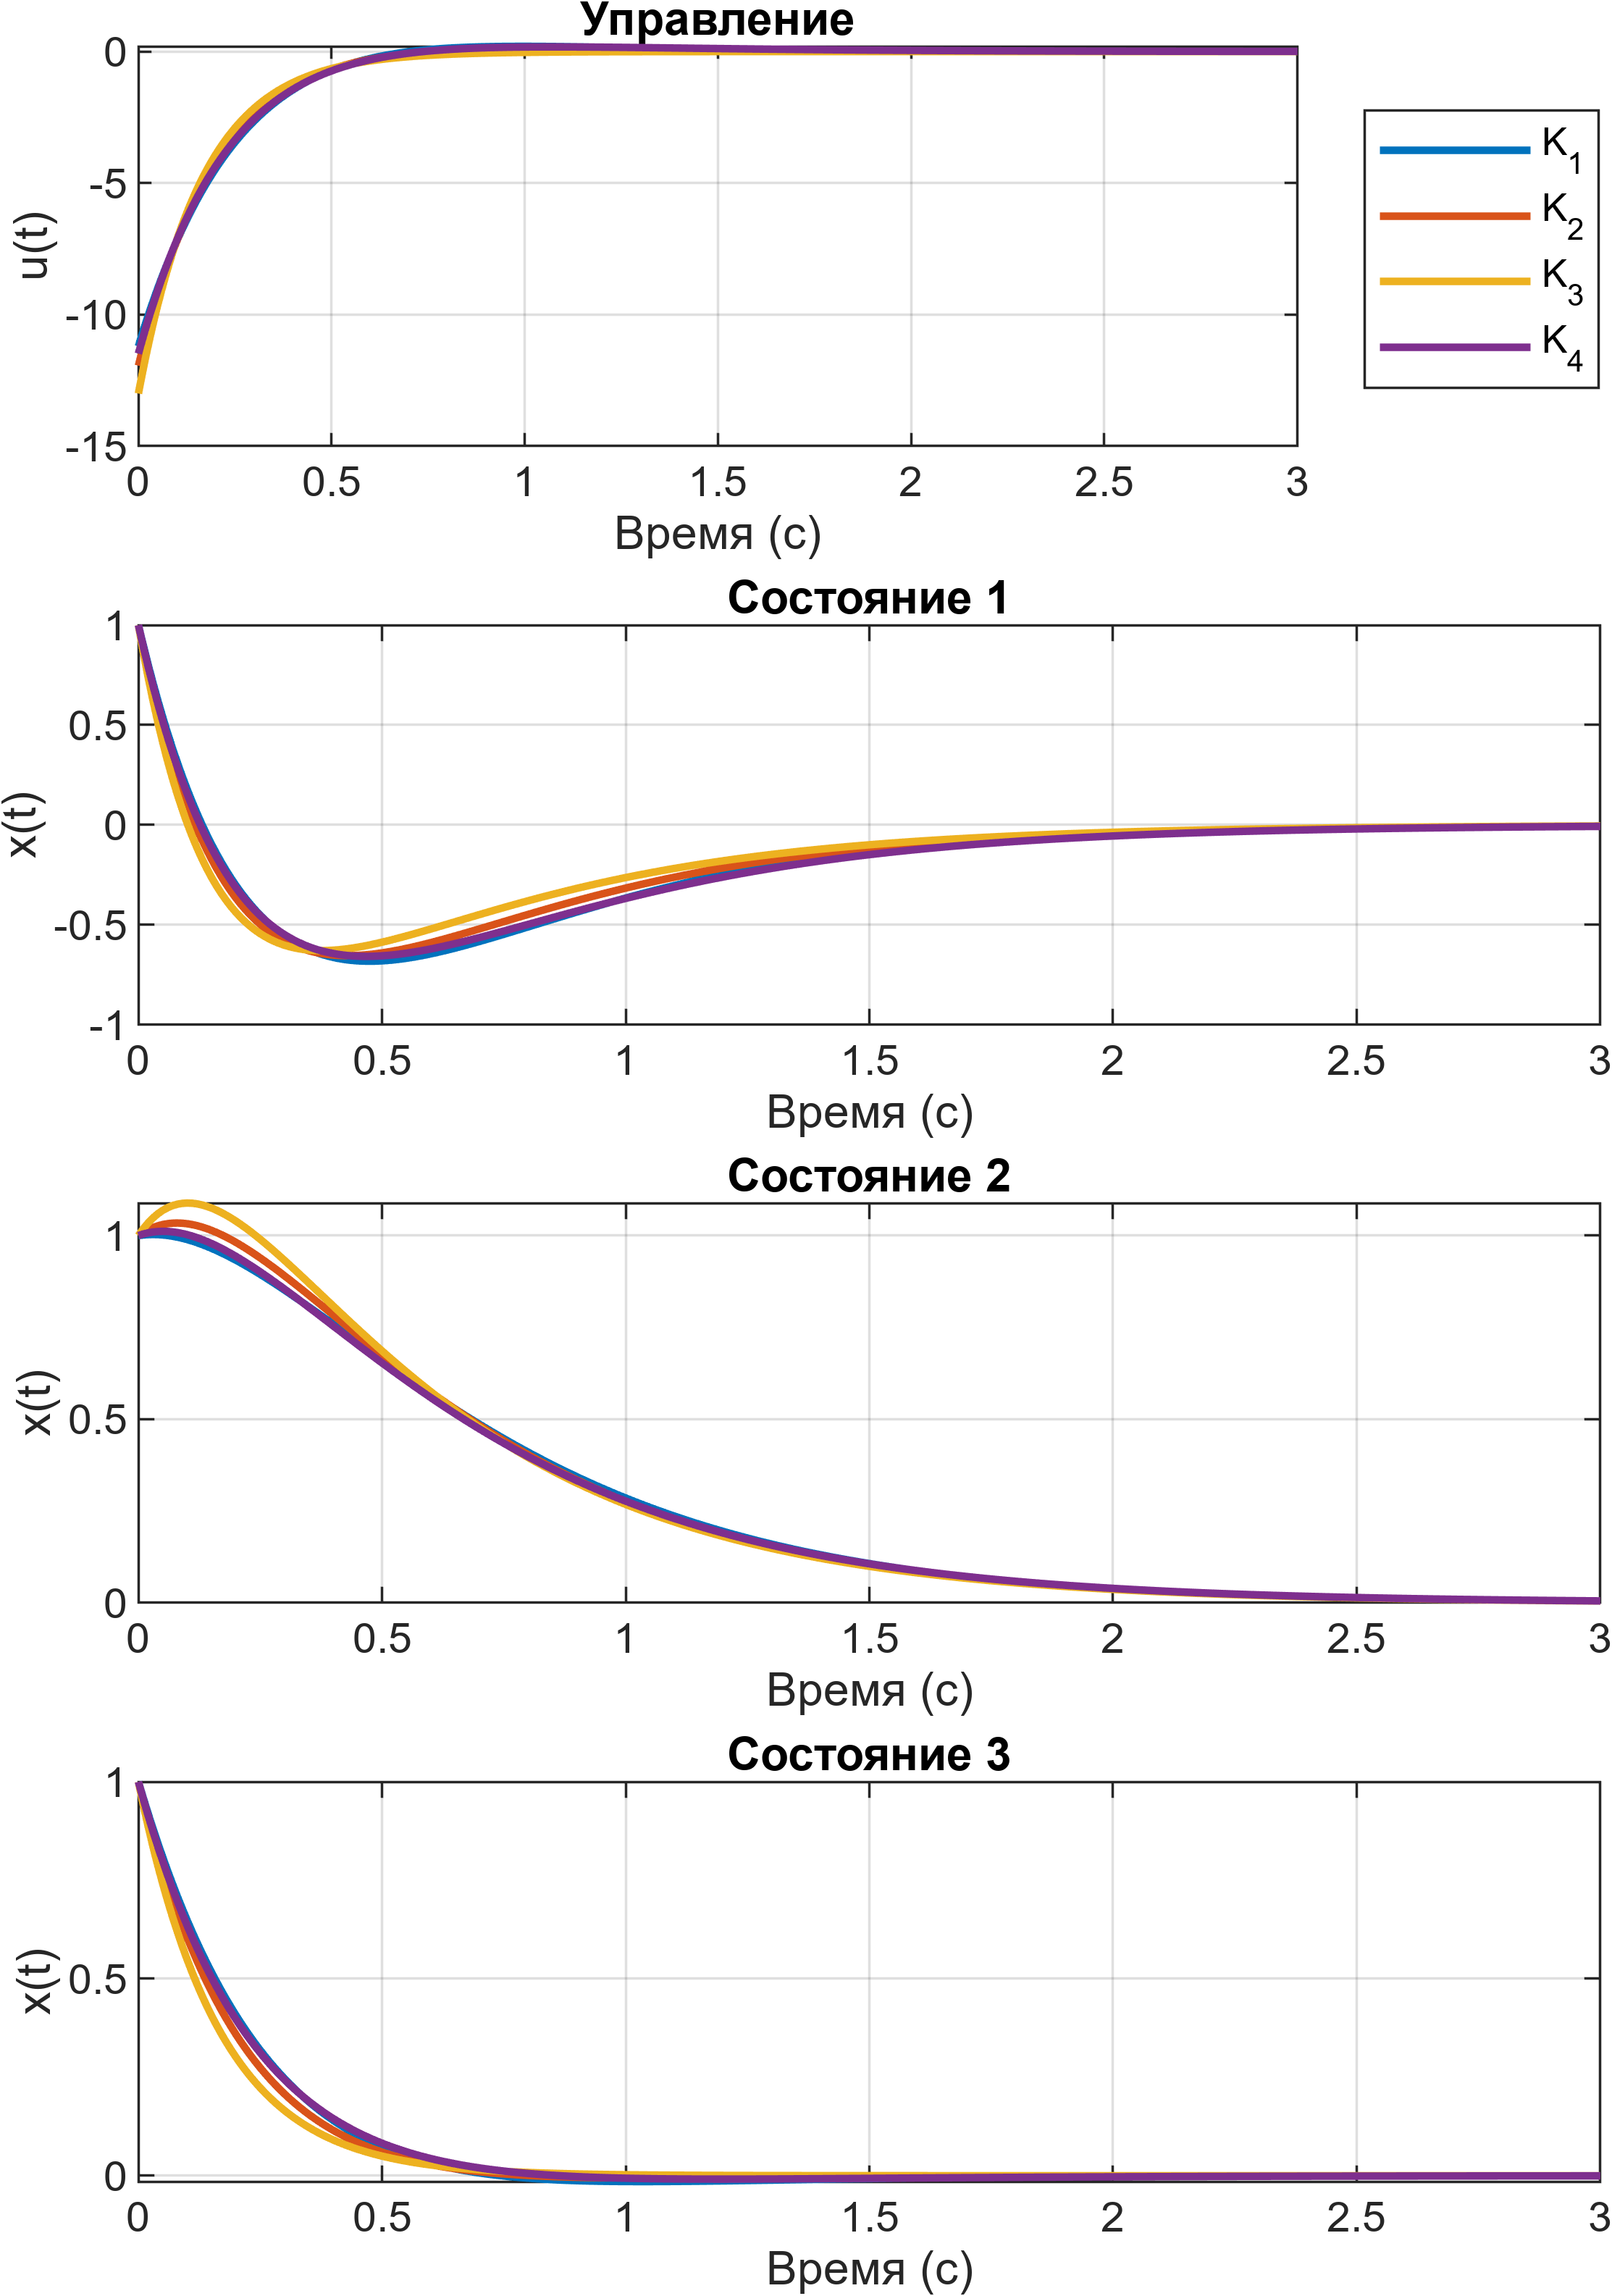
\includegraphics[width=\linewidth]{figs/task31.png}
    \label{fig:riccati2}
\end{figure}


\section{Заключение}

В данной лабораторной работе были рассмотрены различные методы синтеза регуляторов 
и наблюдателей для линейных систем с заданной степенью устойчивости или сходимости 
с минимизацией управления и без. 
Были исследованы подходы на 
основе матричных неравенств типа Ляпунова и матричных уравнений типа Риккати, 
а также синтез регуляторов с качественной экспоненциальной устойчивостью. 
Полученные результаты были подтверждены компьютерным моделированием.